\chapter{Characterization of Finite Automaton Definable Languages}\label{ch-2}

Programming languages can be thought of, in a limited sense, as
conforming to the definition of a language given in Chapter \ref{ch-1}.
We can consider a text file as being one long ``word,'' that is, a
string of characters (including spaces, carriage returns, and so
on). In this sense, each Pascal program can be thought of as a
single word over the ASCII alphabet. We might define the \emph{language}
Pascal as the \emph{set} of all valid Pascal programs (that is, the valid
``words'' are those text files that would compile with no compiler
errors). This and many other languages are too complicated to be
represented by the machines described in Chapter \ref{ch-1}. Indeed,
even reliably matching an unlimited number of begin and end statements
in a file is beyond the capabilities of a DFA.

The goals for this chapter are to develop some tools for identifying
these non-FAD languages and to investigate the underlying structure
of finite automaton definable languages. We begin with the exploration
of the relations that describe that structure.

% 2.1 RIGHT CONGRUENCES
\section{Right Congruences}\label{sec-2.1}

To characterize the structure of FAD languages, we will be dealing
with relations over $\Sigma^*$, that is, we will relate strings to
other strings.  Recall that an \emph{equivalence relation} must be
\emph{reflexive, symmetric}, and \emph{transitive}. The \emph{identity}
relation over $\Sigma^*$, in which each string is related to itself
but to no other string, is an example of an equivalence relation.

The main tool we will need to understand which kinds of languages
can be represented by finite automata is the concept of a \emph{right
congruence}. If we allow the set of all strings that terminate in
some given state to define an \emph{equivalence class}, the states
of a DFA naturally partition $\Sigma^*$ into equivalence classes
(as formally presented later in Definition \ref{dfn-2.4}). Due to
the structure imposed on the machine, these classes have special
relationships that are not found in ordinary equivalence relations.
For example, if $\delta(s, a) = t$, then, given \emph{any} word $x$
in the class corresponding to the state $s$, appending an $\mathbf{a}$
to this word to form $x \mathbf{a}$ is guaranteed to produce a word
listed in the class corresponding to the state $t$. Right congruences,
defined below, allow us to break up $\Sigma^*$ in the same fashion
that a DFA breaks up $\Sigma^*$.

% Definition 2.1
\begin{dfn}\label{dfn-2.1}
Given an alphabet $\Sigma$, a relation $R$ between pairs of strings
$(R \subseteq \Sigma^* \times \Sigma^*)$ is a \emph{\Index{right congruence}} in
$\Sigma^*$ iff the following four conditions hold:
\begin{center}\begin{tabular}{lll}
$(\forall x \in \Sigma^*)$ & $(x\ R\ x)$ & $(R)$ \\
$(\forall x,y \in \Sigma^*)$ & $(x\ R\ y \Rightarrow y\ R\ x)$ & $(S)$ \\
$(\forall x,y,z \in \Sigma^*)$ & $(x\ R\ y \wedge y\ R\ z \Rightarrow x\ R\ z)$
	& $(T)$ \\
$(\forall x,y \in \Sigma^*)$ & $(x \ R\ y \Rightarrow (\forall u \in \Sigma^*)
	(xu \ R\ yu))$ & $(RC)$
\end{tabular}\end{center}
\end{dfn}

Note that if $P$ is a right congruence then the first three conditions imply
that $P$ must be an equivalence relation; for example, if $\Sigma=\{\pmb{a},
\pmb{b}\},\ \pmb{aa}\ P\ \pmb{aa}$ by reflexivity, and if $\langle\pmb{abb},
\pmb{aba}\rangle \in P$, then by symmetry $\langle\pmb{aba},\pmb{abb}\rangle
\in P$, and so forth. Furthermore, if $\pmb{abb}\ P\ \pmb{aba}$, then the right
congruence property guarantees that
\begin{center}\begin{tabular}{ll}
$\pmb{abba}\ P\ \pmb{abaa}$ & if $u = \pmb{a}$ \\ 
$\pmb{abbb}\ P\ \pmb{abab}$ & if $u = \pmb{b}$ \\
$\pmb{abbaa}\ P\ \pmb{abaaa}$ & if $u = \pmb{aa}$ \\
$\pmb{abbbbaabb}\ P\ \pmb{ababbaabb}$ & if $u = \pmb{bbaabb}$ \\
\end{tabular}\end{center}
and so on. Thus, the presence of just one ordered pair in $P$ requires the
existence of many, many more ordered pairs. This might seem to make right
congruences rather rare objects; there are, however, an infinite number of them,
many of them rather simple, as shown by the following examples.

\subsection*{Example 2.1}

Let $\Sigma=\{\pmb{a},\pmb{b}\}$, and let $R$ be defined by $x \ R\ y
\Leftrightarrow |x| - |y|$ is even. It is easy to show that this $R$ is an
equivalence relation (see the exercises) and partitions $\Sigma^*$ into two
equivalence classes: the even-length words and the odd-length words.
Furthermore, $R$ is a right congruence: for example, if $x=\pmb{abb}$ and
$y=\pmb{baabb}$, then $\pmb{abb}\ R\ \pmb{baabb}$, since $|x|-|y|=3-5= -2$, which
is even. Note that for \emph{any} choice of $u$, $\pmb{abb}u\ R\ \pmb{baabb}u$,
since $|xu|-|yu|$ will also be $-2$. Thus $\pmb{abb}u\ R\ \pmb{baabb}u$ for every
choice of $u$. The same is true for any other pair of words $x$ and $y$ that are
related by $R$, and so $R$ is indeed a right congruence.

\subsection*{Example 2.2}

Let $\Sigma=\{\pmb{a},\pmb{b},\pmb{c}\}$, and let $R_2$ be defined by
$x\ R_2 y \Leftrightarrow x$ and $y$ end with the same letter. It is
straightforward to show that $R_2$ is a right congruence (see the exercises)
and partitions $\Sigma^*$ into four equivalence classes: those words ending in
$\pmb{a}$, those words ending in $\pmb{b}$, those words ending in $\pmb{c}$, and
$\{\lambda\}$.

The relation $R_2$ was based on the placement of letters within words, while
Example 2.1 was based solely on the length of the words. The following
definition illustrates a way to produce a relation in $\Sigma^*$ based on a
given set of words $L$.

% Definition 2.2
\begin{dfn}\label{dfn-2.2}
Given an alphabet $\Sigma$, and a language $L \subseteq \Sigma^*$, the
\emph{\Index{relation induced by $L$}} in $\Sigma^*$, denoted by $R_L$, is
defined by
\[ (\forall x,y \in \Sigma^*)(x\ R_L\ y \Leftrightarrow (\forall u \in \Sigma^*)
	(xu \in L \Leftrightarrow yu \in L)) \]
\end{dfn}

\subsection*{Example 2.3}

Let $K$ be the set of all words over $\{\pmb{a},\pmb{b}\}$ that are of odd
length. Those strings that are in $K$ are used to define exactly which pairs of
strings are in $R_K$. For example, we can determine that $\pmb{ab}\ R_K\ 
\pmb{bbaa}$, since it is true that, for any $u \in \Sigma^*$, either
$\pmb{ab}u \notin K$ and $\pmb{bbaa}u \notin K$ (when $|u|$ is even) or
$\pmb{ab}u \in K$ and $\pmb{bbaa}u \in K$ (when $|u|$ is odd). Note that
$\pmb{ab}$ and $\pmb{a}$ are not related by $R_K$, since there are choices for $u$
that would violate the definition of $R_K:\ \pmb{ab}\lambda \notin K$ and yet
$\pmb{a}\lambda \in K$. In this case, $R_K$ turns out to be the same as the
relation $R$ defined in Example 2.1.

Recall that relations are sets of ordered pairs, and thus the claim that these
two relations are equal means that they are equal as sets; an ordered pair
belongs to $R$ exactly when it belongs to $R_K$:
\[ R = R_K\text{ \emph{iff} }(\forall x,y \in \Sigma^*)(x\ R\ y \Leftrightarrow
	x\ R_K\ y) \]
The strings $\pmb{ab}$ and $\pmb{bbaa}$ are related by $R$ in Example 2.1, and they
are likewise related by $R_K$. A similar statement is true for any other pair
that was in the relation $R$; it will be in $R_K$ also. Additionally, it can be
shown that elements that were not in $R$ will not be in $R_K$ either.

Notice that $R_K$ relates more than just the words in $K$; neither $\pmb{ab}$ nor
$\pmb{bbaa}$ belongs to $K$, and yet they were related to each other. This simple
language $K$ happens to partition $\Sigma^*$ into two equivalence classes,
corresponding to the language itself and its complement. Less trivial languages
will often form many equivalence classes. The relation $R_L$ defined by a
language $L$ has all the properties given in Definition \ref{dfn-2.1}.

% Theorem 2.1
\begin{thm}\label{thm-2.1}
Let $\Sigma$ be an alphabet. If $L$ is any language over $\Sigma$ (that is,
$L \subseteq \Sigma^*$), the relation $R_L$ given in Definition \ref{dfn-2.2} must be a
right congruence.

\emph{Proof.} See the exercises.
\end{thm}

Note that the above theorem is very broad in scope: \emph{any} language, no matter
how complex, \emph{always} induces a relation that satisfies all four properties
of a right congruence. Thus, $R_L$ always partitions $\Sigma^*$ into equivalence
classes. One useful measure of the complexity of a language $L$ is the degree to
which it fragments $\Sigma^*$, that is, the number of equivalence classes in
$R_L$.

% Definition 2.3
\begin{dfn}\label{dfn-2.3}
Given an equivalence relation $P$, the \emph{\Index{rank} of} $P$, denoted
$rk(P)$, is defined to be the number of \emph{distinct} (and nonempty)
equivalence classes of $P$.
\end{dfn}

The ranks of the relation in Example 2.3 was 2, since there were two equivalence
classes, the set of even-length words and the set of odd-length words. In
Example 2.2, $rk(R_2)=4$. The rank of $R_L$ can be thought of as a measure of
the complexity of the underlying language $L$. Thus, for $K$ in Example 2.3,
$rk(R_K)=2$, and $K$ might consequently be considered to be a relatively simple
language. Some languages are too complex to be recognized by finite automata;
this relationship will be explored in the subsequent sections.

While the way in which a language gives rise to a partition of $\Sigma^*$ may
seem mysterious and highly nonintuitive, a deterministic finite automaton
naturally distributes the words of $\Sigma^*$ into equivalence classes. The
following definition describes the manner in which a DFA partitions $\Sigma^*$.

% Definition 2.4
\begin{dfn}\label{dfn-2.4}
Given a DFA $M=\langle\Sigma,S,s_0,\delta,F\rangle$, define a relation $R^M$ on
$\Sigma^*$ as follows:
\[ (\forall x,y \in \Sigma^*)(x\ R^M\ y \Leftrightarrow \DBAR(s_0,x) =
	\DBAR(s_0,y)) \]
\end{dfn}

$R^M$ relates all strings that, when starting at $s_0$, wind up at the same
state. It is easy to show that $R^M$ will be an equivalence relation with
(usually) one equivalence class for each state of $M$ (remember that equivalence
classes are by definition nonempty; what type of state might not have an
equivalence class associated with it?). It is also straightforward to show that
the properties of the state transition function guarantee that $R^M$ is in fact
a right congruence (see the exercises).

The equivalence classes of $R^M$ are called \emph{\Index{initial sets}} and will
be of further interest in later chapters. For a DFA $M=\langle\Sigma,S,s_0,
\delta,F\rangle$ and a given state $t$ from $M,\ I(M,t)=\{x\ |\ \DBAR(s_0,x)=t\}$.
This initial set can be thought of as the language accepted by a machine similar
to $M$, but which has $t$ as its only final state. That is, if we define
$M_t=\langle\Sigma,S,s_0,\delta,\{t\}\rangle$, then $I(M,t)=L(M_t)$.

The notation presented here allows a concise method of denoting both relations
defined by languages and relations defined by automata. It is helpful to observe
that even in the absence of context, $R_X$ indicates that a relation based on
the \emph{language} $X$ is being described (since $X$ occurs as a subscript),
while the relation $R^Y$ identifies $Y$ as a \emph{machine} (since Y occurs as a
superscript).

Just as each DFA $M$ gives rise to a right congruence $R^M$, many right
congruences $Q$ can be associated with a DFA, which will be called $A_Q$. It can
be shown that, if some of the equivalence classes of $Q$ are singled out to form
a language $L$, $A_Q$ will recognize $L$.

% Definition 2.5
\begin{dfn}\label{dfn-2.5}
Given a right congruence Q of finite rank and a language $L$ that is the union
of some of the equivalence classes of $Q$, $A_Q$ is defined by
\[ A_Q =\langle\Sigma,S_Q,s_{0_Q},\delta_Q,F_Q\rangle \]
where
\begin{center}\begin{tabular}{l}
$S_Q =\{[x]_Q\ |\ x \in \Sigma^*\}$ \\
$s_{0_Q} = [\lambda]_Q$ \\
$F_Q =\{[x]_Q\ |\ x \in L\}$
\end{tabular}\end{center}
and $\delta_Q$ is defined by
\[ (\forall x \in \Sigma^*)(\forall a \in \Sigma)(\delta_Q([x]_Q,\pmb{a}) =
	[x\pmb{a}]_Q) \]
\end{dfn}

Note that this is a \emph{finite}-state machine since $rk(Q) < \infty$, and that
if $L_1$ were a different collection of equivalence classes of $Q$, $A_Q$ would
remain the same except for the placement of the final states. In other words,
$F_Q$ is the only aspect of this machine that depends on the language $L$ (or
$L_1$). As small as this change might be, it should be noted that $A_Q$ is
defined both by $Q$ and the language $L$. It is left for the reader to show that
$A_Q$ is well-defined and that $L(A_Q)=L$ (see the exercises). The corresponding
statements will be proved in detail in the next section for the important
special case where $Q = R_L$.

\subsection*{Example 2.4}

Let $Q \subseteq \{\pmb{a}\}^* \times \{\pmb{a}\}^*$ be the equivalence relation
with the following equivalence classes:
\begin{center}\begin{tabular}{rcl}
$[\lambda]_Q$\!\!\!\!\! & $=$ &\!\!\!\!\! $\{\lambda\}=\{\lambda\}^0$ \\
$[\pmb{a}]_Q$\!\!\!\!\! & $=$ &\!\!\!\!\! $\{\pmb{a}\}=\{\pmb{a}\}^1$ \\
$[\pmb{aa}]_Q$\!\!\!\!\! & $=$ &\!\!\!\!\! $\{\pmb{a}\}^2 \cup \{\pmb{a}\}^3 \cup \{\pmb{a}\}^4 \cup
	\{\pmb{a}\}^5 \cup \ldots$
\end{tabular}\end{center}
It is easy to show that $Q$ is a right congruence (see the exercises). If $L_1$
were defined to be $[\lambda]_Q \cup [\pmb{a}]_Q$, then $A_Q$ would have the
structure shown in Figure \ref{fig-2.1}a. For the language defined by the different
combination of equivalence classes given by $L_2=[\lambda]_Q \cup [\pmb{aa}]_Q$,
$A_Q$ would look like the DFA given in Figure \ref{fig-2.1}b. This example illustrates
that it is the right congruence $Q$ that establishes the start state and the
transitions, while the language $L$ determines the final state set. It should
also be clear why $L$ must be a union of equivalence classes from $Q$. The
figure shows that a machine with the structure imposed by $Q$ cannot possibly
both reject $\pmb{aaa}$ and accept $\pmb{aaaa}$. Either the entire equivalence class
for $[\pmb{aa}]_Q$ must belong to $L$, or none of the strings from
$[\pmb{aa}]_Q$ can belong to $L$.

% Figure 2.1
\begin{figure}
\centerline{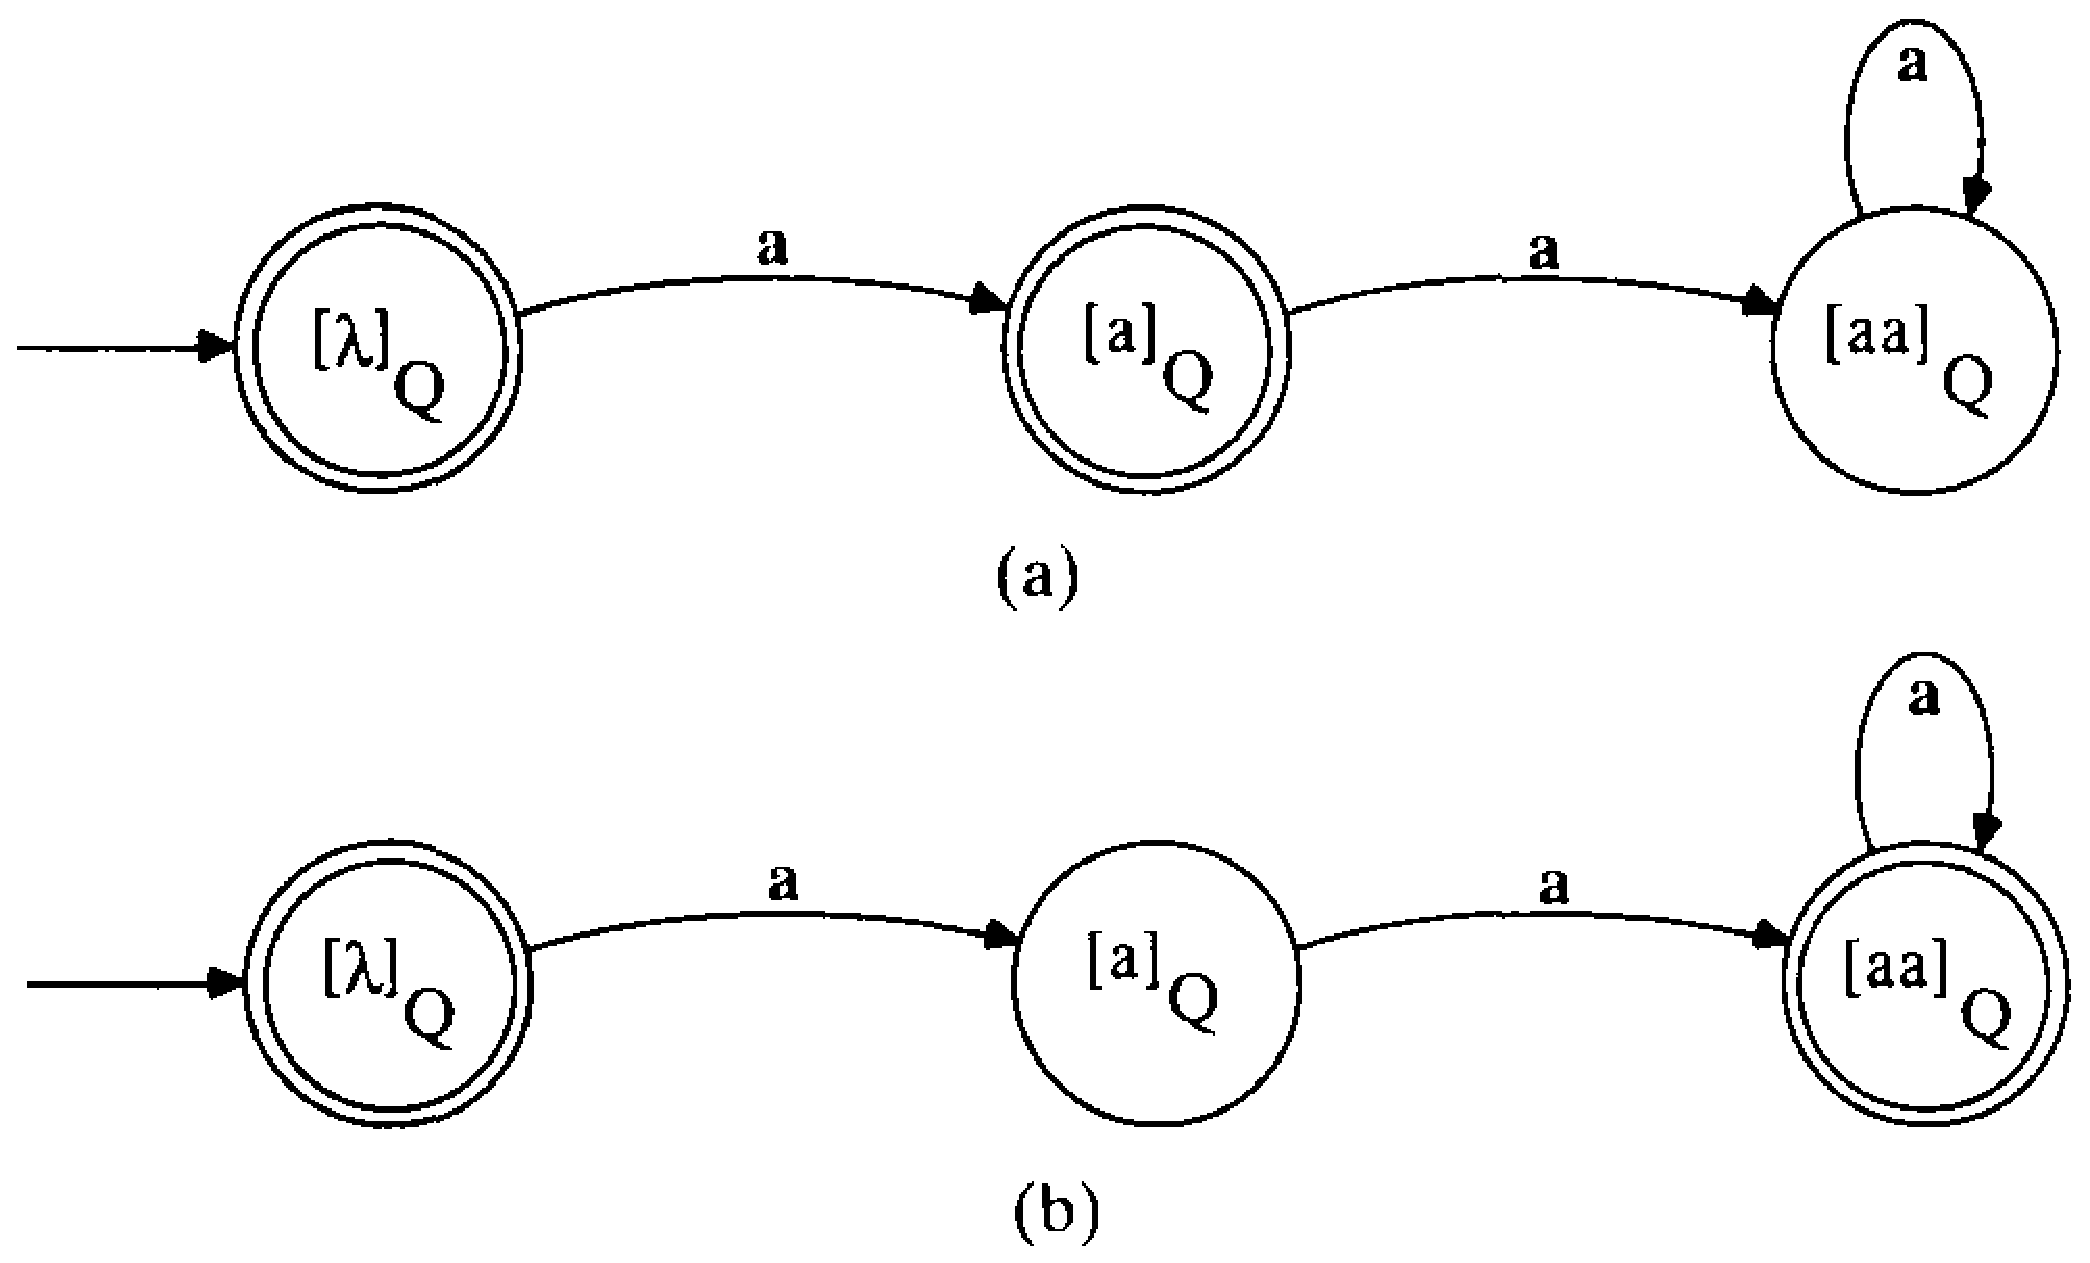
\epsfig{figure=ToFAfigures/fig2-1.eps,width=4in}}
\caption{(a) The automaton for $L_1$ in Example 2.4 (b) The automaton for $L_2$
in Example 2.4}\label{fig-2.1}
\end{figure}

\section{Nerode's Theorem}\label{sec-2.2}

In this section, we will show that languages that partition $\Sigma^*$ into a
finite number of equivalence classes can be represented by finite automata,
while those that yield an infinite number of classes would require a machine
with an infinite number of states.

\subsection*{Example 2.5}

The language $K$ given in Example 2.3 can be represented by a finite automaton
with two states; all words that have an even number of letters eventually wind
up at state $s_0$, while all the odd words are taken by \DBAR\ to $s_1$. This
machine is shown in Figure \ref{fig-2.2}.

It is no coincidence that these states split up the words of $\Sigma^*$ into the
same equivalence classes that $R_K$ does. There is an intimate relationship
between languages that can be represented by a machine with a finite number of
states and languages that induce right congruences with a finite number of
equivalence classes, as outlined in the proof of the following theorem.

% Figure 2.2
\begin{figure}
\centerline{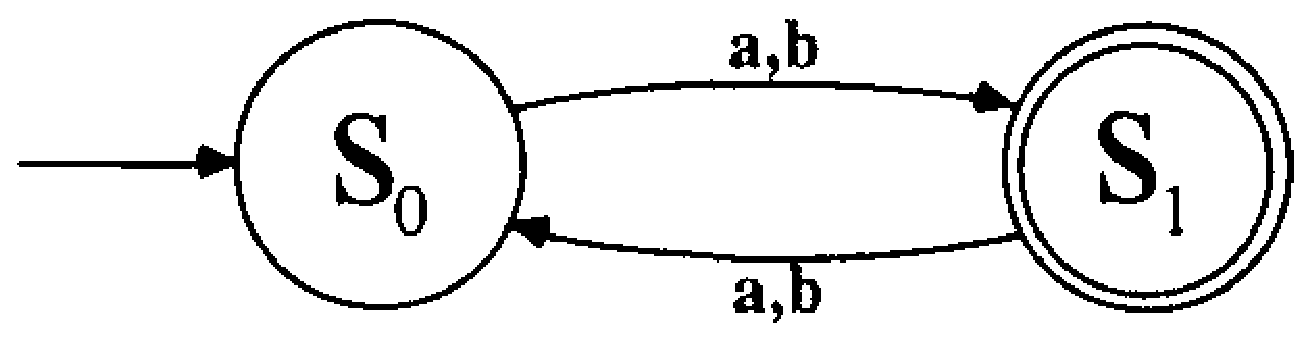
\epsfig{figure=ToFAfigures/fig2-2.eps,width=2.5in}}
\caption{The DFA discussed in Example 2.5}\label{fig-2.2}
\end{figure}

% Theorem 2.2
\begin{thm}\label{thm-2.2}
{\bf Nerode's Theorem}. Let $L$ be a language over an alphabet $\Sigma$; the
following statements are all equivalent:
\begin{enumerate}
\item $L$ is FAD.
\item There exists a right congruence $R$ on $\Sigma^*$ for which $L$ is the
(possibly empty) union of some of the equivalence classes of $R$ and $rk(R) <
	\infty$.
\item $rk(R_L) < \infty$.
\end{enumerate}

\emph{Proof.} Because of the transitivity of $\Rightarrow$, it will be
sufficient to show only the three implications (1) $\Rightarrow$ (2), (2) 
$\Rightarrow$ (3), and (3) $\Rightarrow$ (1), rather than all six of them.

\emph{Proof of} (1) $\Rightarrow$ (2): Assume (1); that is, let $L$ be FAD. Then
there is a machine that accepts $L$; that is, there exists a finite automaton
$M=\langle\Sigma,S,s_0,\delta,F\rangle$ such that $L(M) = L$. Consider the
relation $R^M$ on $\Sigma^*$ based on this machine $M$ as given in Definition
\ref{dfn-2.4}: $(\forall x,y \in \Sigma^*)(x\ R^M\ y \Leftrightarrow \DBAR(s_0,x) =
\DBAR(s_0,y))$.

This $R^M$ will be the relation $R$ we need to prove (2). For each $s \in S$,
consider $I(M,s)=\{x \in \Sigma^*\ |\ \DBAR(s_0,x) = s\}$, which represents all
strings that wind up at state $s$ (from $s_0$). Note that it is easy to define
automata for which it is impossible to reach certain states from the start
state; for such states, $I(M,s)$ would be empty. Then $\forall s \in S,\ I(M,s)$
is either an equivalence class of $R^M$ or $I(M,s)=\emptyset$. Since there is at
most one equivalence class per state, and there are a finite number of states,
it follows that $rk(R^M)$ is also finite: $rk(R^M) \leq \|S\| < \infty$.

However, we have
\[ L=L(M) = \{x \in \Sigma^*\ |\ \DBAR(s_0,x) \in F\}= \bigcup\limits_{f \in F}
	\{x \in \Sigma^*\ |\ \DBAR(s_0,x)=f\} = \bigcup\limits_{f \in F} I(M,f) \]
That is, $L$ is the union of some of the equivalence classes of the right
congruence $R^M$, and $R^M$ is indeed of finite rank, and hence (2) is
satisfied. Thus (1) $\Rightarrow$ (2).

\emph{Proof of} (2) $\Rightarrow$ (3): Assume that (2) holds; that is, there is
a right congruence $R$ for which $L$ is the union of some of the equivalence
classes of the right congruence $R$, and $rk(R) < \infty$. Note that we no
longer have (1) as an assumption; there is no machine (as yet) associated with
$L$.

{\bf Case 1}: It could be that $L$ is the empty union; that is, that
$L=\emptyset$. In this case, it is easy to show that $R_L$ has only one
equivalence class ($\Sigma^*$), and thus $rk(R_L) = 1 < \infty$ and (3) will be
satisfied.

{\bf Case 2}: In the nontrivial case, $L$ is the union of one or more of the
equivalence classes of the given right congruence $R$, and it is possible to
show that this $R$ must then be closely related to the $R_L$ induced by the
original language $L$. In particular, for any strings $x$ and $y$,
\begin{center}\begin{tabular}{rcl}
$x R\ y$ & $\Rightarrow$ & (since $R$ is a right congruence) \\
$(\forall u \in \Sigma^*)(xu\ R\ yu)$ & $\Rightarrow$ & (by definition of
	$[\ ]$) \\
$(\forall u \in \Sigma^*)([xu]_R = [yu]_R)$ & $\Rightarrow$ & (by definition of
	$L$ as a union of $[\ ]$'s) \\\
$(\forall u \in \Sigma^*)(xu \in L \Leftrightarrow yu \in L)$ & $\Rightarrow$ &
	(by definition of $R_L$) \\
$x\ R_L\ y$ &&
\end{tabular}\end{center}
$(\forall x \in \Sigma^*)(\forall y \in \Sigma^*)(x\ R\ y \Rightarrow x\ R_L\ y)$
means that $R$ refines $R_L$, and thus each equivalence class of $R$ is entirely
contained in an equivalence class of $R_L$; that is, each equivalence class of
$R_L$ must be a union of one or more equivalence classes of $R$. Thus, there are
more equivalence classes in $R$ than in $R_L$, and so $rk(R_L) \leq rk(R)$. But by
hypothesis, $rk(R)$ is finite, and so $R_L$ must be of finite rank also, and
(3) is satisfied. Thus, in either case, (2) $\Rightarrow$ (3).

\emph{Proof of} (3) $\Rightarrow$ (1): Assume now that condition (3) holds; that
is, $L$ is a language for which $R_L$ is of finite rank. Once again, note that
all we know is that $R_L$ has a finite number of equivalence classes; we do not
have either (1) or (2) as a hypothesis. Indeed, we wish to show (1) by proving
that $L$ is accepted by some finite automaton. We will base the structure of
this automaton on the right congruence $R_L$, using Definition \ref{dfn-2.5} with
$Q = R_L$. $A_{R_L}$ is then defined by
\begin{align*}
& A_{R_L} =\langle\Sigma,S_{R_L},s_{0_{R_L}},\delta_{R_L},F_{R_L}\rangle \\
\intertext{where}
& S_{R_L}=\{[x]_{R_L}|\ x \in \Sigma^*\} \\
& s_{0_{R_L}} = [\lambda]_{R_L} \\
& F_{R_L} =\{[x]_{R_L}|\ x \in L\}
\end{align*}
and $\delta_{R_L}$ is defined by
\[ (\forall x \in \Sigma^*)(\forall\pmb{a}\in\Sigma)(\delta_{R_L}([x]_{R_L},
	\pmb{a}) = [x\pmb{a}]_{R_L}) \]
The basic idea in this construction is to define one state for each equivalence
class in $R_L$, use the equivalence class containing $\lambda$ as the start
state, use those classes that were made up of words in $L$ as final states, and
define $\delta$ in a natural manner. We claim that this machine is really a
well-defined finite automaton and that it does behave as we wish it to; that is,
the language accepted by $A_{R_L}$ really is $L$. In other words, $L(A_{R_L})=L$.

First, note that $S_{R_L}$ is a finite set, since [by the only assumption we
have in (3)] $R_L$ consists of only a finite number of equivalence classes. It
can be shown that $F_{R_L}$ is well defined; if $[z]_{R_L}=[y]_{R_L}$, then
either (both $z \in L$ and $y \in L$) or (neither $z$ nor $y$ belong to $L$)
(why?). The reader should show that $\delta_{R_L}$ is similarly well defined;
that is, if $[z]_{R_L}=[y]_{R_L}$, it follows that $\delta_{R_L}$ is forced to
also take both transitions to the same state $([z\pmb{a}]_{R_L}=[y\pmb{a}]_{R_L})$.
Also, a straightforward induction on $|y|$ shows that the rule for
$\delta_{R_L}$ extends to a similar rule for $\DBAR_{R_L}$:
\[ (\forall x \in \Sigma^*)(\forall y \in \Sigma^*)(\DBAR_{R_L}([x]_{R_L},y) =
	[xy]_{R_L}) \]
With this preliminary work out of the way, it is possible to easily show that
$L(A_{R_L}) = L$. Let $x$ be any element of $\Sigma^*$. Then
\begin{center}\begin{tabular}{rcl}
$x \in L(A_{R_L})$ & $\Leftrightarrow$ & (by definition of $L$) \\
$\DBAR_{R_L}(s_{0_{R_L}},x) \in F_{R_L}$ & $\Leftrightarrow$ & (by definition of
	$s_{0_{R_L}}$) \\
$\DBAR_{R_L}([\lambda]_{R_L},x) \in F_{R_L}$ & $\Leftrightarrow$ & (by
	definition of $\DBAR_{R_L}$ and induction) \\
$[\lambda x]_{R_L} \in F_{R_L}$ & $\Leftrightarrow$ & (by definition of $\lambda$) \\
$[x]_{R_L} \in F_{R_L}$ & $\Leftrightarrow$ & (by definition of $F_{R_L}$) \\
$x \in L$ &&
\end{tabular}\end{center}
Consequently, $L$ is exactly the language accepted by this finite automaton; so
$L$ must be FAD, and (1) is satisfied. Thus (3) $\Leftrightarrow$ (1). We have
therefore come full circle, and all three conditions are equivalent.
\end{thm}

The correspondence described by Nerode's theorem can best be illustrated by
an example.

\subsection*{Example 2.6}

% Figure 2.3
\begin{figure}
\centerline{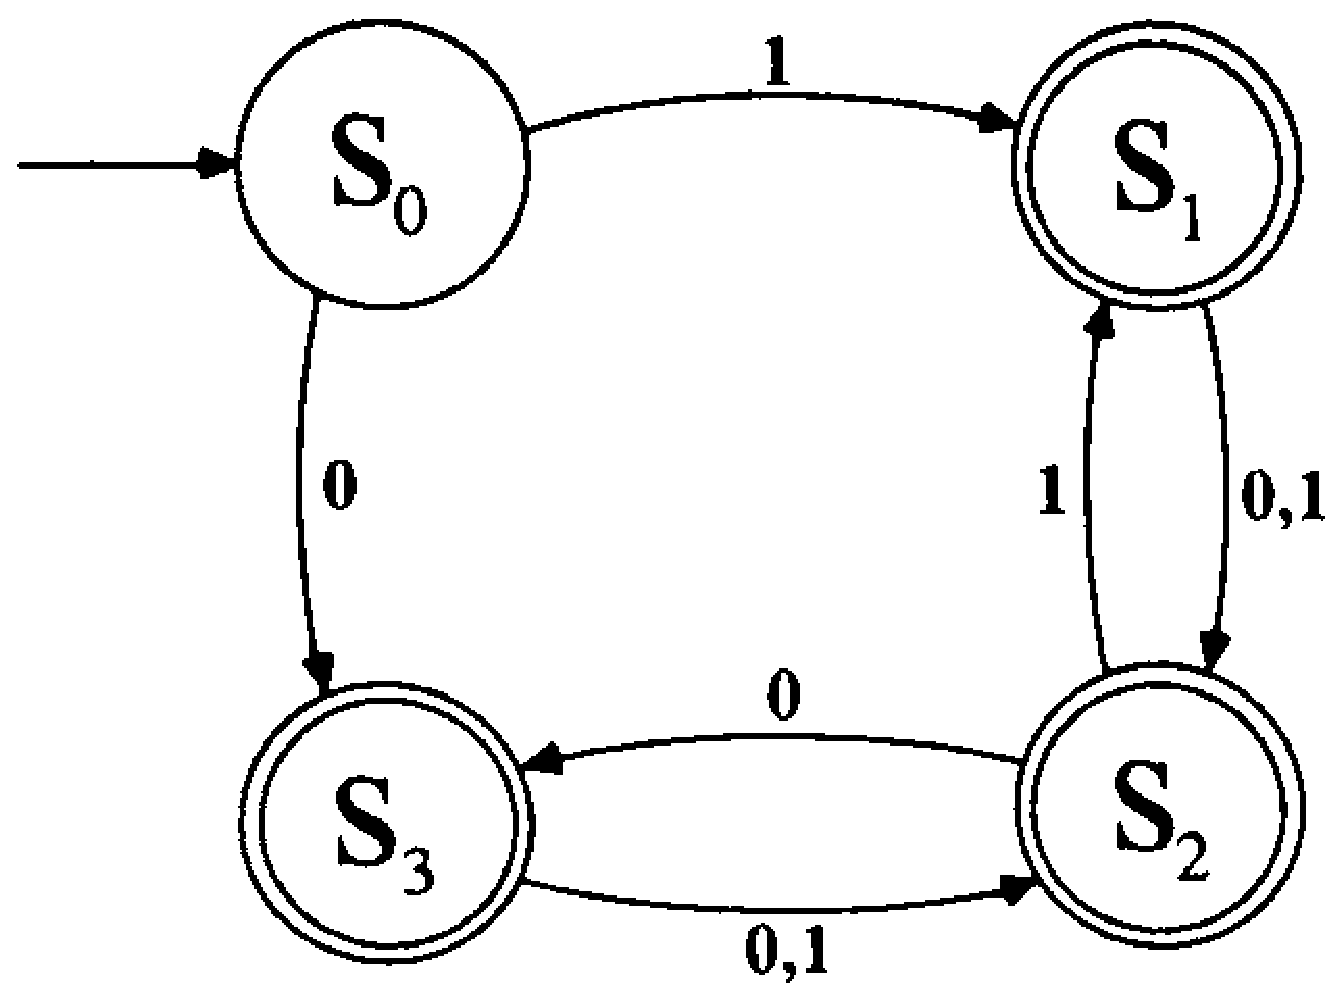
\epsfig{figure=ToFAfigures/fig2-3.eps,width=2.5in}}
\caption{The DFA $N$ discussed in Example 2.6}\label{fig-2.3}
\end{figure}

Let $L$ be the following FAD language: $L=\Sigma^* - \{\lambda\} = \Sigma^+$.
There are many finite automata that accept $L$, one of which is the DFA given in
Figure \ref{fig-2.3}. This four-state machine gives rise to a four-equivalence class right
congruence as described in (1) $\Rightarrow$ (2), where
\begin{center}\begin{tabular}{rclcl}
$[\lambda]_{R^N}$ & $=$ & $I(N,s_0)$ & $=$ & $\{\lambda\}$, since $\lambda$ is
	the only string that ends up at $s_0$ \\
$[\pmb{1}]_{R^N}$ & $=$ & $I(N,s_1)$ & $=$ & $\{y|\ |y|$ is odd, and $y$ ends
	with a $\pmb{1}\} = \{z\ |\DBAR(s_0,z) = s_1\}$ \\
$[\pmb{11}]_{R^N}$ & $=$ & $I(N,s_2)$ & $=$ & $\{y|\ |y|$ is even$\}-\{\lambda\}
	= \{z\ |\DBAR(s_0,z) = s_2\}$ \\
$[\pmb{000}]_{R^N}$ & $=$ & $I(N,s_3)$ & $=$ & $\{y|\ |y|$ is odd, and $y$ ends
	with a $\pmb{0}\} = \{z\ |\DBAR(s_0,z) = s_3\}$
\end{tabular}\end{center}
Note that $L$ is indeed $I(N,s_1) \cup I(N,s_2)  \cup I(N,s_3)$ which is the
union of all the equivalence classes that correspond to final states in $N$, as
required by (2). To illustrate (2) $\Rightarrow$ (3), let $R$ be the equivalence
relation $R^N$ defined above, let $L$ again be $\Sigma^+$, and note that (2) is
satisfied: $L=[\pmb{1}]_R \cup [\pmb{11}]_R \cup [\pmb{000}]_R$, the union of
3 of the equivalence classes of a right congruence of rank 4 (which is finite).

As in the proof of (2) $\Rightarrow$ (3), $R_L$ is refined by $R$, but in this
case $R$ and $R_L$ are not equal. All the relations from $R$ still hold, such as
$\pmb{11}\ R\ \pmb{1111}$, so $\pmb{11}\ R_L\ \pmb{1111}$; $\pmb{0}\ R\ 
\pmb{000}$, and thus $\pmb{0}\ R_L\ \pmb{000}$, and so forth. It can also be
shown that $\pmb{11}\ R_L\ \pmb{000}$, even though $\pmb{11}$ and $\pmb{000}$
were not related by $R$ (apply the definition of $R_L$ to convince yourself of
this). Thus, everything in $[\pmb{11}]_R$ is related by $R_L$ to everything in
$[\pmb{000}]_R$; that is, all the strings belong to the same equivalence class
\emph{of} $R_L$, even though they formed separate equivalence classes \emph{in}
$R$. It may at first appear strange, but the fact that there are \emph{more} relations
in $R_L$ means that there are \emph{fewer} equivalence classes in $R_L$ than in
$R$. Indeed, $R_L$ has only two equivalence classes, $\{\lambda\}$ and $L$. In
this case, three equivalence classes of $R$ collapse to form one large
equivalence class of $R_L$. Thus $\{\lambda\}=[\lambda]_{R_L}=[\lambda]_R$ and
$L=[\pmb{11}]_{R_L}=[\pmb{1}]_R \cup [\pmb{11}]_R \cup [\pmb{000}]_R$ and, as we
were assured by (2) $\Rightarrow$ (3), $R$ refines $R_L$.

To illustrate (3) $\Rightarrow$ (1), let's continue to use the $L$ and $R_L$
given above. Since $R_L$ is of rank 2, we are assured of finding a two-state
machine that will accept $L$. $A_{R_L}$ in this case would take the form of the
automaton $P$ displayed in Figure \ref{fig-2.4}. In this DFA, for example,
$\delta([\pmb{11}]_{R_L},\pmb{0})=[\pmb{110}]_{R_L}=[\pmb{11}]_{R_L}$, and
$[\lambda]_{R_L}$ is the start state. $[\pmb{11}]_{R_L}$ is a final state since
$\pmb{11} \in L$. Verify that this machine accepts all words except $\lambda$;
that is, $L(A_{R_L}) = L$.

\subsection*{Example 2.7}

% Figure 2.4
\begin{figure}
\centerline{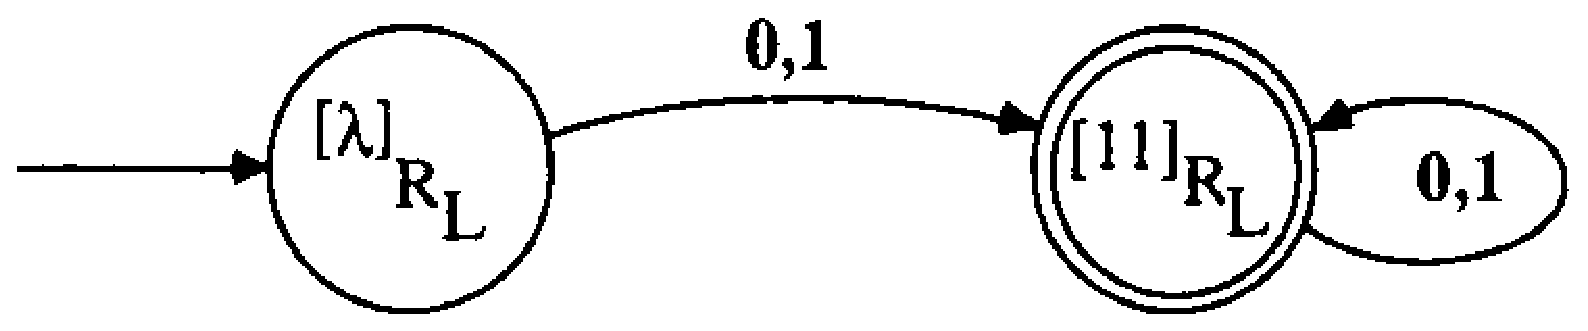
\epsfig{figure=ToFAfigures/fig2-4.eps,width=3.0in}}
\caption{The DFA $P$ discussed in Example 2.6}\label{fig-2.4}
\end{figure}

Assume $Q$ is defined to be the right congruence $R$ given in Example 2.6, and
$L$ is again $\Sigma^+$, which is the union of three of the equivalence classes
of $Q:\ [\pmb{1}]_Q,\ [\pmb{11}]_Q$, and $[\pmb{000}]_Q$. The automaton $A_Q$ is
given in Figure \ref{fig-2.5}.

% Figure 2.5
\begin{figure}
\centerline{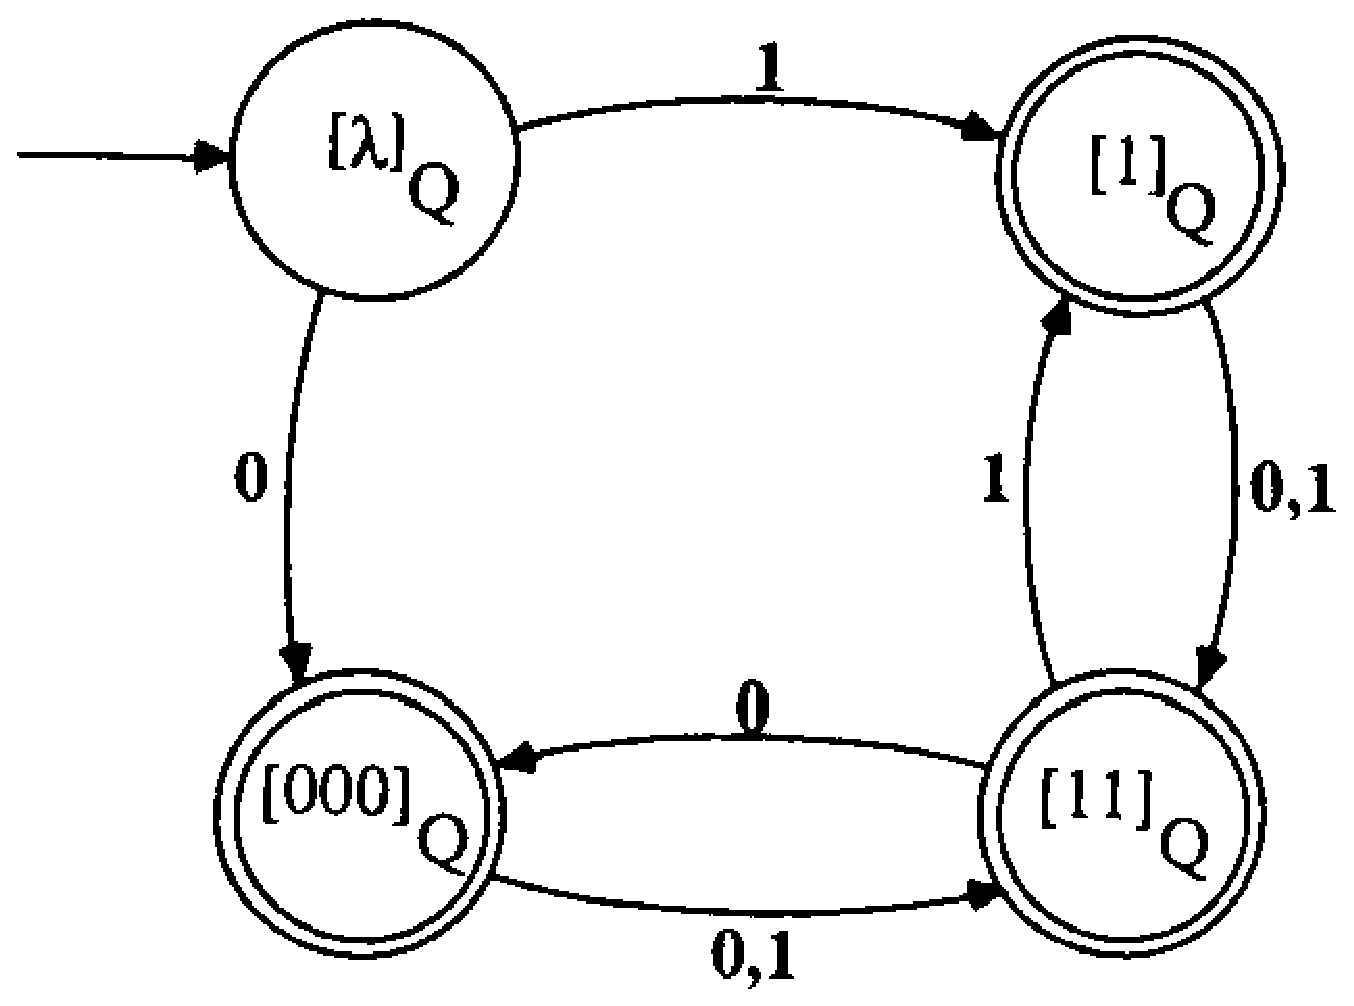
\epsfig{figure=ToFAfigures/fig2-5.eps,width=2.5in}}
\caption{The automaton discussed in Example 2.7}\label{fig-2.5}
\end{figure}

If we were instead to begin with the same language $L$, but use the two-state
machine $P$ at the end of Example 2.6 to represent $L$, we would find that $L$
would consist of only one equivalence class, $R^P$ would have only two
equivalence classes, and $R^P$ would in this case be the same as $R_L$ (see the
exercises). $R^P$ turns out to be as simple as $R_L$ because the machine we
started with was as ``simple'' as we could get and still represent $L$. In
Chapter \ref{ch-3} we will characterize the idea of a machine being ``as simple as
possible,'' that is, \emph{\Index{minimal}}.

The two machines given in Example 2.6 accept the same language. It will be
convenient to formalize this notion of distinct machines ``performing the same
task,'' and we therefore make the following definition.

% Definition 2.6
\begin{dfn}\label{dfn-2.6}\index{equivalent!DFAs}
Two DFAs $A$ and $B$ are \emph{equivalent} iff $L(A) = L(B)$.
\end{dfn}

\subsection*{Example 2.8}

The DFAs $N$ from Example 2.6 and $A_Q$ from Example 2.7 are equivalent since
$L(N) = \Sigma^+ = L(A_Q)$ .

% Definition 2.7
\begin{dfn}\label{dfn-2.7}
A DFA $A=\langle\Sigma,S_A,s_{0_A},\delta_A,F_A\rangle$ is \emph{\Index{minimal}}
iff for every DFA $B=\langle\Sigma,S_B,s_{0_B},\delta_B,F_B\rangle$ for which
$L(A) = L(B),\ |S_A| \leq |S_B|$.
\end{dfn}

An automaton is therefore minimal if no equivalent machine has fewer states.

\subsection*{Example 2.9}

The DFA $N$ from Example 2.6 is clearly not minimal since the automaton $P$
from Example 2.6 is equivalent and has fewer states than $N$. The techniques
from Chapter \ref{ch-3} can be used to verify that the automaton $P$ from Example 2.6
is minimal. More importantly, minimization techniques will be explored in
Chapter \ref{ch-3} that will allow an optimal machine (like this $P$) to be produced
from an inefficient automaton (like $N$).

\section{Pumping Lemmas}\label{sec-2.3}

As you have probably noticed by now, finding $R_L$ and counting the equivalence
classes is not a very practical way of verifying that a suspected language
cannot be defined by a finite automaton. It would be nice to have a better way
to determine if a given language is unwieldy. The \emph{\Index{pumping lemma}}
will supply us with such a technique. It is based on the observation that if
your automaton processes a ``long enough'' word it must eventually visit (at
least) one state more than once.

Let $A=\langle\Sigma,S,s_0,\delta,F\rangle$, and consider starting at some state
$s$ and processing a word $x$ of length 5. We will pass through state $s$ and
perhaps five other states, although these states may not all be distinct if we
visit some of them repeatedly while processing the five letters in $x$; thus the
total will be six states (or less). Note that if $A$ has 10 states $(\|S\|=10)$
and $|x| = 12$ we cannot go to 13 \emph{different} states while processing $x$;
(at least) one state must be visited more than once.

% Figure 2.6
\begin{figure}
\centerline{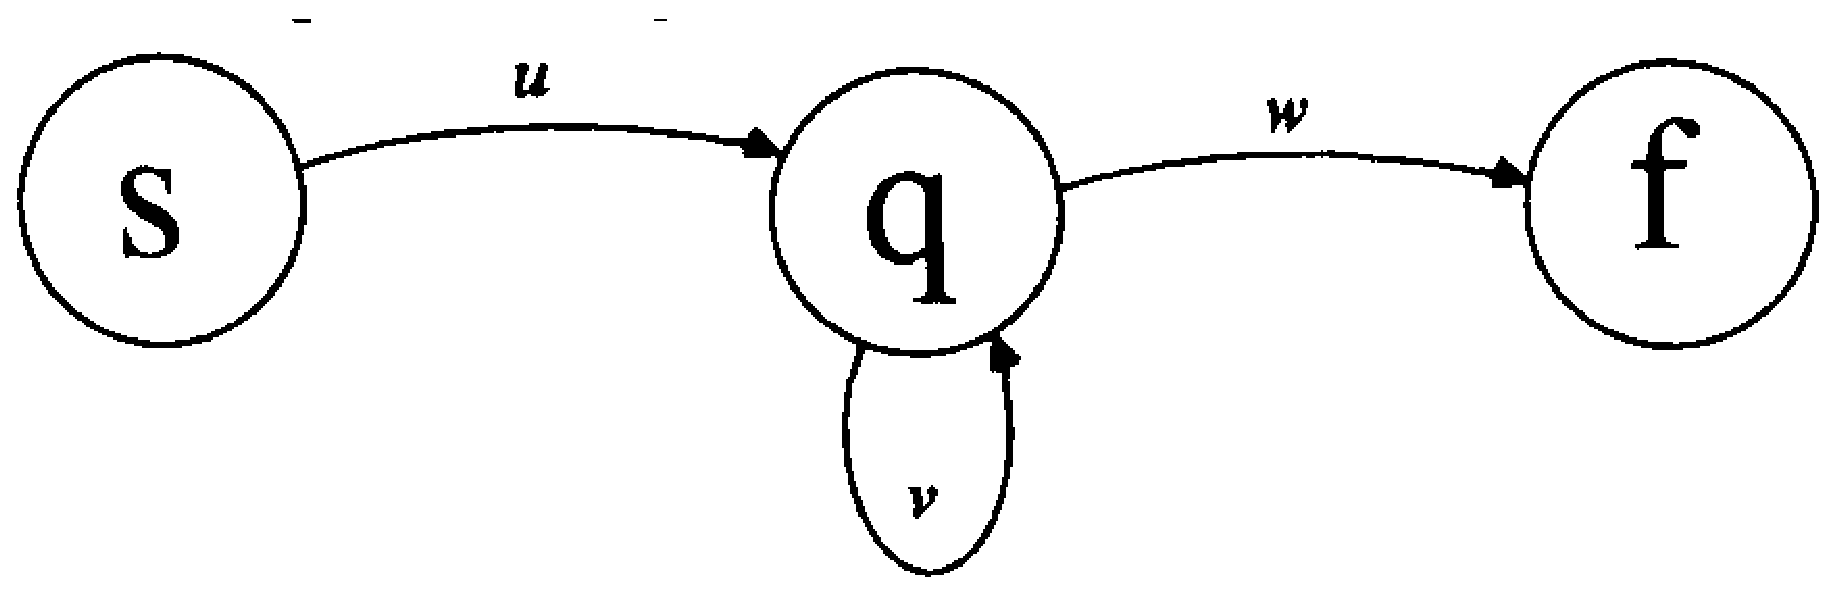
\epsfig{figure=ToFAfigures/fig2-6.eps,width=4.0in}}
\caption{A path with a loop}\label{fig-2.6}
\end{figure}

In general, if $n=\|S\|$, then any string $x$ whose length is equal to or
greater than $n$ must pass through some state $q$ twice while being processed by
$A$, as shown in Figure \ref{fig-2.6}. Here the arrows are meant to represent the path
taken while processing \emph{several} letters, and the intermediate states are not
shown. The strings $u$, $v$, and $w$ are defined as
\begin{center}\begin{tabular}{l}
$u$ = first few letters of $x$ that take us to the state $q$ \\
$v$ = next few letters of $x$ that will again take us back to $q$ \\
$w$ = rest of the string $x$
\end{tabular}\end{center}
Then, with $x = uvw$, we have $\DBAR(s,u) = q,\ \DBAR(s,uv) = q$, and in fact
$\DBAR(q,v) = q$. Also, $\DBAR(s,x) = \DBAR(s,uvw) =$ $f$ and $\DBAR(q,w)= f$, as
is clear from the diagram. Now consider the string $uw$, that is, the string $x$
with the $v$ part ``removed'':
\begin{center}\begin{tabular}{rcl}
$\DBAR(s,uw)$ & $=$ & $\DBAR(\DBAR(s,u),w)\qquad\text{(why?)}$ \\
& $=$ & $\DBAR(q,w)$ \\
& $=$ & $f$
\end{tabular}\end{center}
That is, the string $uw$ winds up in the same place $uvw$ does; this is
illustrated in Figure \ref{fig-2.7}a. Note that a similar thing happens if $uv^2 w$ is
processed:
\begin{center}\begin{tabular}{rcl}
$\DBAR(s,uvvw)$ & $=$ & $\DBAR(\DBAR(s,u),vvw)$ \\
& $=$ & $\DBAR(q,vvw)$ \\
& $=$ & $\DBAR(\DBAR(q,v),vw)$ \\
& $=$ & $\DBAR(q,vw)$ \\
& $=$ & $\DBAR(\DBAR(q,v),w)$ \\
& $=$ & $\DBAR(q,w)$ \\
& $=$ & $f$
\end{tabular}\end{center}
This behavior is illustrated in Figure \ref{fig-2.7}b.

% Figure 2.7
\begin{figure}
\centerline{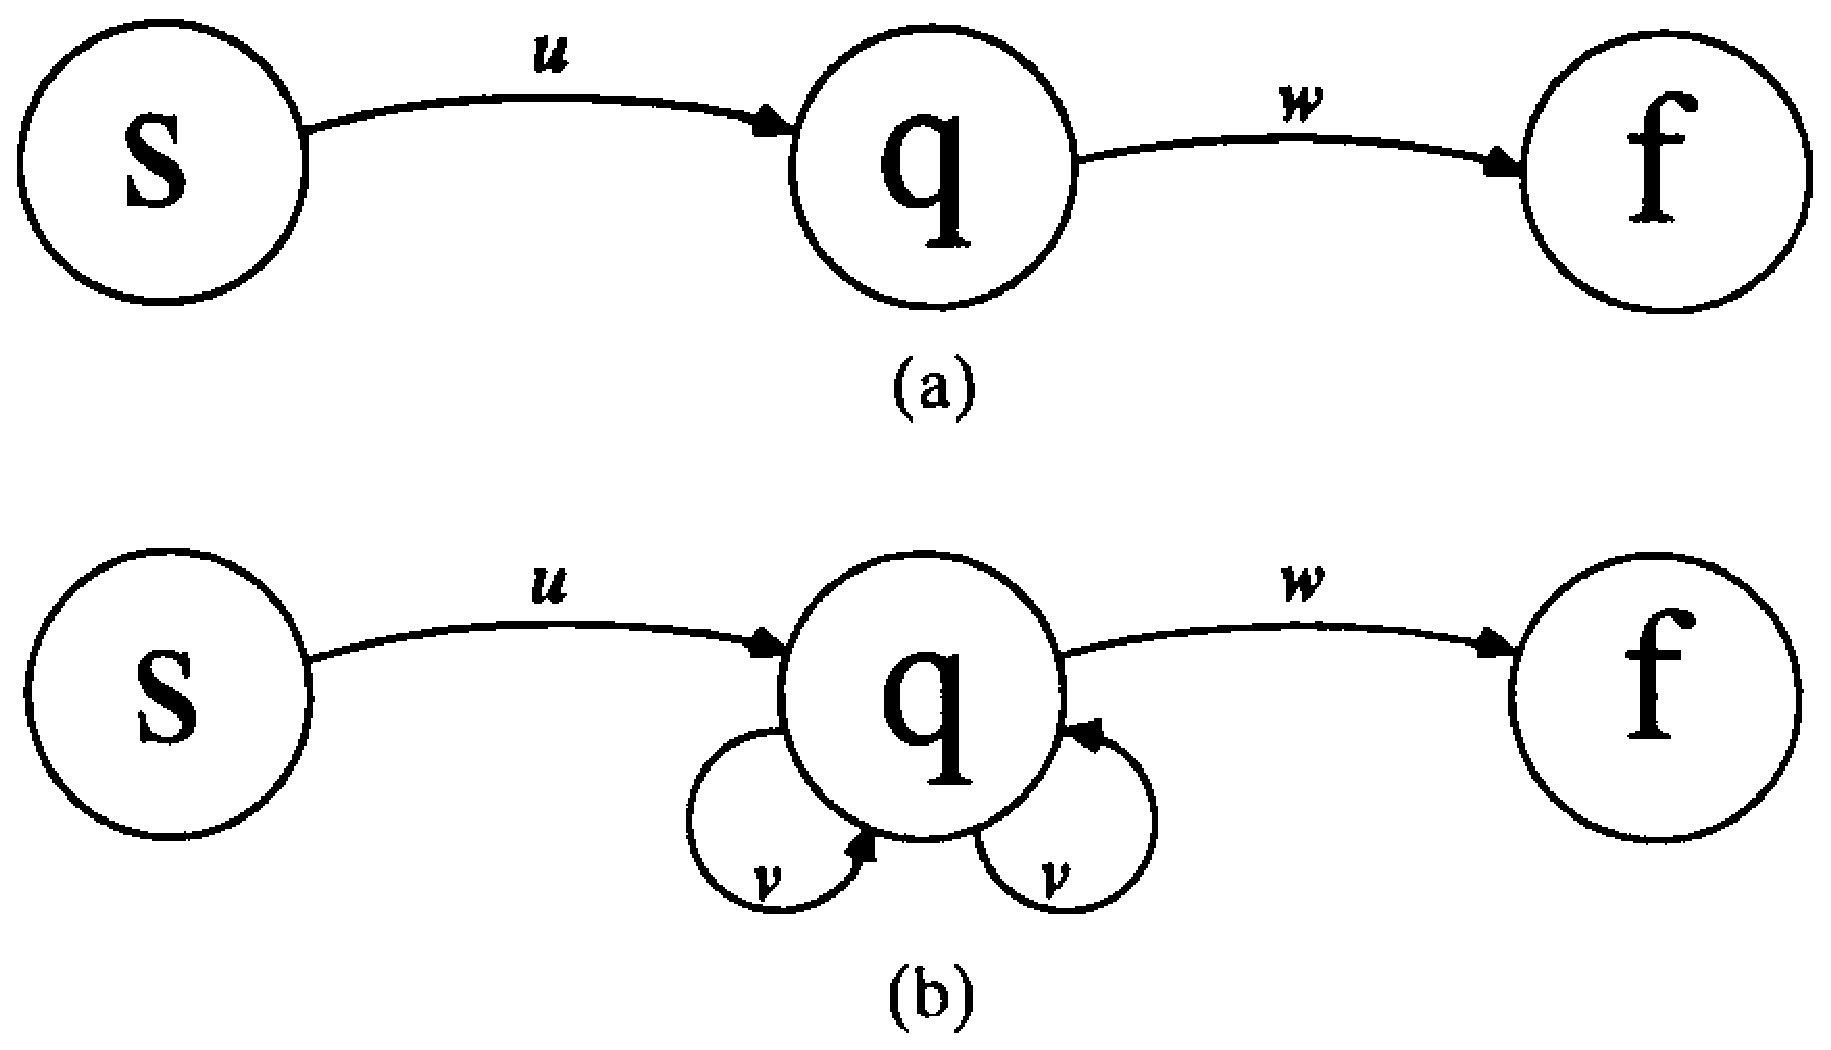
\epsfig{figure=ToFAfigures/fig2-7.eps,width=4.0in}}
\caption{(a) The path that bypasses the loop (b) The path that traverses the
loop twice}\label{fig-2.7}
\end{figure}

In general, it can be proved by induction that $(\forall i \in \NN)(\DBAR(s,
uv^i\!w)=\text{f}=\DBAR(s,uvw))$. Notice that we do reach $q$ two \emph{distinct} times,
which implies that the string $v$ contains at least one letter; that is,
$|v| \geq 1$. Also, after the first $n$ letters of $x$, we must have already
repeated a state, and thus some state $q$ can be found such that $|uv| \leq n$.
If $s$ happens to be the start state $s_0$ and $f$ is a final state, we have
now shown that: If $A=\langle\Sigma,S,s_0,\delta,F\rangle$, where $\|S\| = n$,
then, given any string $x=\pmb{a}_1\pmb{a}_2\pmb{a}_3 \ldots \pmb{a}_m$, where
$m \geq n$ and $\DBAR(s_0,x)= f \in F$ [which implies $x \in L(A)$], the states
$\DBAR(s_0,\lambda),\DBAR(s_0,\pmb{a}_1),\DBAR(s_0,\pmb{a}_1\pmb{a}_2),
\DBAR(s_0,\pmb{a}_1\pmb{a}_2\pmb{a}_3), \ldots ,\DBAR(s_0,\pmb{a}_1\pmb{a}_2
\ldots \pmb{a}_n)$ cannot all be distinct, and so $x$ can be broken up into
strings $u$, $v$, and $w$ such that
\begin{center}\begin{tabular}{rcl}
$x$ & $=$ & $uvw$ \\
$|uv|$ & $\leq$ & $n$ \\
$|v|$ & $\geq$ & $1$
\end{tabular}\end{center}
and $(\forall i \in \NN)(\DBAR(s_0,uv^i\!w)=$f$)$, that is, $(\forall i \in \NN)
(uv^i\!w \in L(A))$. In other words, given any ``long'' string in $L(A)$, there is
a part of the string that can be ``pumped'' to produce even longer strings in
$L(A)$.

Thus, if $L$ is FAD, there exists an automaton (with a finite number $n$ of
states), and thus for some $n\in\NN$, the above statement should hold. We have
just proved what is generally known as the \emph{pumping lemma}, which we now
state formally.

% Theorem 2.3: The Pumping Lemma
\begin{thm}\label{thm-2.3}
{\bf The Pumping Lemma.} Let $L$ be an FAD language over $\Sigma^*$. Then
$(\exists n \in \NN)(\forall x \in L \ni |x| \geq n)(\exists u,v,w \in
\Sigma^*) \ni$
\begin{center}\begin{tabular}{rcl}
$x$ & $=$ & $uvw$ \\
$|uv|$ & $\leq$ & $n$ \\
$|v|$ & $\geq$ & $1$
\end{tabular}\end{center}
and
\[ (\forall i \in \NN)(uv^i\!w \in L). \]

\emph{Proof.} Given above.
\end{thm}

\subsection*{Example 2.10}

Let $E$ be the set of all even-length words over $\{\pmb{a},\pmb{b}\}^*$. There is
a two-state machine that accepts $E$, so $E$ is FAD, and the pumping lemma
applies if $n$ is, say, 5. Then $\forall x \ni |x| > 5$, if $x = 
\pmb{a}_1\pmb{a}_2\pmb{a}_3\ldots\pmb{a}_j \in E$ (that is, $j$ is even), we can
choose $u=\lambda,\ v=\pmb{a}_1\pmb{a}_2$, and $w=\pmb{a}_3\pmb{a}_4\ldots
\pmb{a}_j$. Note that $|uv|= 2 \leq 5$, $|v| = 2 \geq 1$, and $|uv^iw|=j+2(i-1)$,
which is even, and so $(\forall i \in \NN)(uv^iw \in E)$.

If Example 2.10 does not appear truly exciting, there is good reason: The
pumping lemma is generally not applied to FAD languages! (\emph{Note:} We \emph{will}
see an application later.) The pumping lemma is often applied to show languages
are \emph{not} FAD (by proving that the language does not satisfy the pumping lemma).
Note that the contrapositive of Theorem \ref{thm-2.3} is:

% Theorem 2.4
\begin{thm}\label{thm-2.4}
Let $L$ be a language over $\Sigma^*$. {\bf If} \\
$(\forall n \in \NN)(\exists x \in L \ni |x| \geq n)(\forall u,v,w \in
\Sigma^* \ni x = uvw,|uv| \leq n, |v| \geq 1)(\exists i \in \NN \ni uv^i\!w
\notin L)$, \\
{\bf then} $L$ is not FAD.

\emph{Proof.} See the exercises.
\end{thm}

\subsection*{Example 2.11}

Consider $L_4=\{y \in \{\pmb{0},\pmb{1}\}^*|\ |y|_{\pmb{0}} = |y|_{\pmb{1}}\}$. We will
use Theorem \ref{thm-2.4} to show $L_4$ is not FAD: Let $n$ be given, and choose $x =
\pmb{0}^n \pmb{1}^n$. Then $x \in L_4$, since $|x|_{\pmb{0}} = n = |x|_{\pmb{1}}$. It should be
observed that $x$ must be dependent on $n$, and we have \emph{no} control over
$n$ (in particular, $n$ cannot be replaced by some constant; similarly, while
$i$ may be chosen to be a convenient fixed constant, a proof that covers all possible
combinations of $u$, $v$, and $w$ must be given).

Note that this choice of $x$ is ``long enough'' in that $|x| = 2n \geq n$, as
required by Theorem \ref{thm-2.4}. For \emph{any} combination of $u,\ v,\ w \in \Sigma^*$ such
that $x = uvw,\ |uv| \leq n,\ |v| \geq 1$, we hope to find a value for $i$ such
that $uv^iw \notin L_4$. Since $|uv| \leq n$ and the first $n$ letters of $x$ are
all zeros, this narrows down the choices for $u,\ v$, and $w$. They must be of
the form $u = \pmb{0}^j$ and $v = \pmb{0}^k$ (since $|uv| \leq n$ and $x$ starts
with $n$ zeros), and $w$ must be the ``rest of the string'' and look something
like $w=\pmb{0}^m \pmb{1}^n$. The constraints on $u,\ v$, and $w$ imply that
$j + k \leq n,\ k \geq 1$, and $j + k + m = n$. If $i = 2$, we have that
$uv^2w = \pmb{0}^{n+k} \pmb{1}^n \notin L_4$ (why?). Thus, by Theorem \ref{thm-2.4}, $L_4$ is not FAD
[or, alternately, because the conclusion of the pumping lemma (Theorem \ref{thm-2.3}) does
\emph{not} hold, $L_4$ cannot be FAD].

It is instructive to endeavor to build a DFA that attempts to recognize the
language $L_4$. As you begin to see what such a machine must look like, it
will become clear that no matter how many states you add (that is, no matter how
large $n$ becomes) there will always be some strings (``long'' strings) that
would require even more states. Your construction may also suggest what the
equivalence classes of $R_{L_4}$ must look like (see the exercises). How many
equivalence classes are there? (You should be able to answer this last question
without referring to any constructions.)

A similar argument can be made to show that no DFA can recognize the set of all
fully parenthesized infix expressions (see the exercises). Matching parentheses,
like matching $\pmb{0}$s and $\pmb{1}$s in the last example, requires unlimited
storage. We have seen that DFAs are adequate vehicles for pattern matching and
token identification, but a more complex model is clearly needed to implement
functions like the parsing of arithmetic expressions. \emph{Pushdown automata},\index{pushdown automaton} discussed in Chapter \ref{ch-10}, augment the finite memory with an unbounded
stack, allowing more complex languages to be recognized.

Intuitively, we would not expect \emph{finite}-state machines to be able to
differentiate between arbitrarily long integers. While \emph{modular}
arithmetic, which only differentiates between a finite number of remainders,
should be representable by finite automata, unrestricted arithmetic is likely to
be impossible. For example, $\{\pmb{a}^i\pmb{b}^j\pmb{c}^k\ |\ i,j,k \in \NN$ and
$i + j = k\}$ cannot be recognized by any DFA, while the language
$\{\pmb{a}^i\pmb{b}^j\pmb{c}^k\ |\ i,j,k \in \NN$ and $i + j \equiv k \bmod{3}\}$ is
FAD. Checking whether two numbers are relatively prime is likewise too difficult
for a DFA, as shown by the proof in the following example.

\subsection*{Example 2.12}

Consider $L=\{\pmb{a}^i\pmb{b}^j\ |\ i,j \in \NN$ and $i$ and $j$ are relatively
prime$\}$. We will use Theorem \ref{thm-2.4} to show $L$ is not FAD: Let $n$ be given, and
choose a prime $p$ larger than $n + 1$ (we can be assured such a $p$ exists
since there are an infinite number of primes). Let $x=\pmb{a}^p\pmb{b}^{(p-1)!}$.
Since $p$ has no factors other than $1$ and $p$, it has no nontrivial factor in
common with $(p-1) \cdot (p-2) \cdot \ldots \cdot 3 \cdot 2 \cdot 1$, and so $p$
and $(p-1)!$ are relatively prime, which guarantees that $x \in L$. The length
of $x$ is clearly greater than $n$, so Theorem \ref{thm-2.3} should apply, which implies
that there must exist a combination $u,v,w \in \Sigma^*$ such that $x = uvw,
|uv| \leq n, |v| \geq 1$; we hope to find a value for $i$ such that $uv^iw \in L$.
Since $|uv| \leq n$ and the first $n$ letters of $x$ are all $\pmb{a}$s, there
must exist integers $j,\ k$, and $m$ for which $u=\pmb{a}^j$ and $v=\pmb{a}^k$,
and $w$ must be the ``rest of the string''; that is, $w=\pmb{a}^m
\pmb{b}^{(p-1)!}$. The constraints on $u,\ v$, and $w$ imply that $j + k \leq n$,
$k \geq 1$, and $j + k + m = p$. If $i = 0$, we have that $uv^{0} w =
\pmb{a}^{p-k}\pmb{b}^{(p-1)!}$. But $p-k$ is a number between $p-1$ and $p-n$
and hence must match one of the nontrivial factors in $(p-1)!$, which means that
$uv^{0} w \notin L$ (why?). Therefore, Theorem \ref{thm-2.3} has been violated, so $L$
could not have been FAD.

The details of the basic argument used to prove the pumping lemma can be varied
to produce other theorems of a similar nature: for example, when processing $x$,
there must be a state $q'$ repeated within the last $n$ letters. This gives rise
to the following variation of the pumping lemma.

% Theorem 2.5
\begin{thm}\label{thm-2.5}
Let $L$ be a FAD language over $\Sigma^*$. Then
\[ (\exists n \in \NN)(\forall x \in L \ni |x| \geq n)(\exists u,v,w \in
	\Sigma^*) \ni \]
\begin{center}\begin{tabular}{rcl}
$x$ & $=$ & $uvw$ \\
$|vw|$ & $\leq$ & $n$, \\
$|v|$ & $\geq$ & $1$ \\
\end{tabular}\end{center}
and
\[ (\forall i \in \NN)(uv^iw \in L) \]

\emph{Proof.} See the exercises.
\end{thm}

The new condition $|vw| \leq n$ reflects the constraint that some state must be
repeated within the last $n$ letters. The contrapositive of Theorem \ref{thm-2.5} can be
useful in demonstrating that certain languages are not FAD. By repeating our
original reasoning while assuming the string $x$ takes us to a \emph{non}final state,
we obtain yet another variation.

% Theorem 2.6
\begin{thm}\label{thm-2.6}
Let $L$ be a FAD language over $\Sigma^*$. Then
\[ (\exists n \in \NN)(\forall x \notin L \ni |x| \geq n)(\exists u,v,w \in
	\Sigma^*) \ni \]
\begin{center}\begin{tabular}{rcl}
$x$ & $=$ & $uvw$ \\
$|uv|$ & $\leq$ & $n$ \\
$|v|$ & $\geq$ & $1$ \\
\end{tabular}\end{center}
and
\[ (\forall i \in \NN)(uv^iw \notin L) \]

\emph{Proof.} See the exercises.
\end{thm}

Notice that Theorem \ref{thm-2.6} guarantees that if one ``long'' string is
{\em not} in the
language then there is an entire sequence of strings that cannot be in the
language. There are some examples of languages in the exercises where Theorem
\ref{thm-2.4} is hard to apply, but where Theorem \ref{thm-2.5} (or Theorem \ref{thm-2.6}) is appropriate.

When $i = 0$, the pumping lemma states that given a ``long'' string ($uvw$) in
$L$ there is a shorter string ($uw$) that is also in $L$. If this new string is
still of length greater than $n$, the pumping lemma can be reapplied to find a
still shorter string, and so on. This technique is the basis for proving the
following theorem.

% Theorem 2.7
\begin{thm}\label{thm-2.7}
Let $M$ be an $n$-state DFA accepting $L$. Then
\[ (\forall x \in L \ni x = \pmb{a}_1\pmb{a}_2 \ldots \pmb{a}_m,\text{ and }m
	\geq n)(\exists\text{ an increasing sequence }i_1,i_2, \ldots ,i_j) \]
for which $\pmb{a}_{i_1}\pmb{a}_{i_2} \ldots \pmb{a}_{i_j} \in L$, and $j < n$.

\emph{Proof.} See the exercises.
\end{thm}

Note that $\pmb{a}_{i_1}\pmb{a}_{i_2} \ldots \pmb{a}_{i_j}$ represents a string
formed by ``removing'' letters from perhaps several places in $x$, and that this
new string has length less than $n$. Theorem \ref{thm-2.7} can be applied in areas that do
not initially seem to relate to DFAs. Consider an arbitrary right congruence $R$
of (finite) rank $n$. It can be shown that each equivalence class of $R$ is
guaranteed to contain a representative of length less than $n$. For example,
consider the relation $R$ given by
\begin{center}\begin{tabular}{rcl}
$[\lambda]_R$ & $=$ & $\{\lambda\}$ \\
$[\pmb{11111}]_R$ & $=$ & $\{y\ |\ \ |y|\text{ is odd, and $y$ ends with a }
	\pmb{1}\}$ \\
$[\pmb{0101}]_R$ & $=$ & $\{y\ |\ \  |y|\text{ is even and }|y| > 0\}$ \\
$[\pmb{00000}]_R$ & $=$ & $\{y\ |\ \  |y|\text{ is odd, and $y$ ends with a }
	\pmb{0}\}$
\end{tabular}\end{center}
In this relation, $rk(R) = 4$, and appropriate representatives of length less
than 4 are $\lambda,\ \pmb{1},\ \pmb{11}$, and $\pmb{100}$, respectively. That
is, $[\lambda]_R = [\lambda]_R,\ [\pmb{1}]_R = [\pmb{11111}]_R,\ [\pmb{11}]_R
= [\pmb{0101}]_R$, and $[\pmb{100}]_R = [\pmb{00000}]_R$. By constructing a DFA
based on the right congruence $R$, Theorem \ref{thm-2.7} can be used to prove that every
equivalence class of $R$ has a ``short'' representative (see the exercises).

We have seen that deterministic finite automata are limited in their cognitive
powers, that is, there are languages that are too complex to be recognized by
DFAs. When only a finite set of previous histories can be distinguished, the
resulting languages must have a certain repetitious nature. Allowing automata to
instead have an infinite number of states is uninteresting for several reasons.
On the practical side, it would be inconvenient (to say the least) to physically
construct such a machine. Infinite automata are also of little theoretical
interest as they do not distinguish between simple and complex languages: {\em any}
language can be accepted by the infinite analog of a DFA. With an infinite
number of states available, the state transition diagrams can look like trees,
with a unique state corresponding to each word in $\Sigma^*$. The states
corresponding to desired words can simply be made final states.

More reasonable enhancements to automata will be explored later. Non-determinism
will be presented in Chapter \ref{ch-4}, and machines with extended capabilities will be
defined and investigated in Chapters \ref{ch-10} and \ref{ch-11}.

\section*{Exercises}

\begin{enumerate}[{2.}1.]
\item Let $\Sigma=\{\pmb{a},\pmb{b},\pmb{c}\}$. Show that the relation $\Psi
\subseteq \Sigma^* \times \Sigma^*$ defined by
\[ x\ \Psi\ y \Leftrightarrow |x|-|y|\text{ is odd} \]
is \emph{not} a right congruence. (Is it an equivalence relation?)

\item Let $\Sigma=\{\pmb{a},\pmb{b},\pmb{c}\}$. Consider the relation $Q
\subseteq \Sigma^* \times \Sigma^*$ defined by
\[ x\ Q\ y \Leftrightarrow |x|_{\pmb{a}} - |y|_{\pmb{a}} \equiv 0 \bmod{3} \]
\begin{enumerate}
\item Show that $Q$ is an equivalence relation.
\item Assume that part (a) is true, and show that $Q$ is a right congruence.
\end{enumerate}

\item Let $\Sigma=\{\pmb{a},\pmb{b},\pmb{c}\}$. Find all languages $L$ such that
$rk(R_L) = 1$. Justify your conclusions.

\item Let $P \subseteq \{\pmb{0},\pmb{1}\}^* \times \{\pmb{0},\pmb{1}\}^*$ be
the equivalence relation with the following equivalence classes:
\begin{center}\begin{tabular}{rcl}
$[\lambda]_P$ & $=$ & $\{\lambda\} = \{\pmb{0},\pmb{1}\}^0$ \\
$[\pmb{1}]_P$ & $=$ & $\{\pmb{0},\pmb{1}\} = \{\pmb{0},\pmb{1}\}^1$ \\
$[\pmb{00}]_P$ & $=$ & $\{\pmb{0},\pmb{1}\}^2 \cup \{\pmb{0},\pmb{1}\}^3 \cup
	\{\pmb{0},\pmb{1}\}^4 \cup \{\pmb{0},\pmb{1}\}^5 \cup \ldots$
\end{tabular}\end{center}
Show that $P$ is a right congruence.

\item For the relation $P$ defined in Exercise 2.4, find all languages $L \ni
R_L = P$.

\item For the relation $Q$ defined in Exercise 2.2, find all languages $L \ni
R_L = Q$.

% NOTE: Having trouble getting the spacing on the \not portion of the !Q
% operator
\item Let $\Sigma=\{\pmb{a},\pmb{b}\}$. Define the relation $Q$ by $\lambda Q
\lambda$, and $(\forall x \not= \lambda)(\lambda \not\!\! Q x)$, and
\[ (\forall x \not= \lambda)(\forall y \not= \lambda )[x\ Q\ y \Leftrightarrow
	(|x|\text{ is even }\wedge |y|\text{ is even})\vee(|x|\text{ is odd }
	\wedge |y|\text{ is odd})], \]
which implies that
\[ (\forall x \not= \lambda)(\forall y \not= \lambda)[x \not\!\! Q\ y
	\Leftrightarrow (|x|\text{ is even }\wedge |y|\text{ is odd})\vee(|x|
	\text{ is odd} \wedge |y|\text{ is even})]. \]
\begin{enumerate}
\item Show that $Q$ is a right congruence. and list the equivalence classes.
\item Define $L=[\lambda]_Q \cup [\pmb{aa}]_Q$. Find a simple description for
$L$, and list the equivalence classes of $R_L$. (Note that $Q$ does refine
$R_L$.)
\item Draw a machine with states corresponding to the equivalence classes of
$Q$. Arrange the final states so that the machine accepts $L$ (that is, find
$A_Q$).
\item Draw $A_{R_L}$.
\item Consider the machine in part (c) above ($A_Q$). Does it look like
$A_{R_L}$? Can you rearrange the final states in $A_Q$ (producing a new language
$K$) so that $A_{R_K}$ looks like your new $A_Q$? Illustrate.
\item Consider all eight languages found by taking unions of equivalence classes
from $Q$, and see which ones would satisfy the criteria of part (e).
\end{enumerate}

\item Let $\Sigma=\{\pmb{a}\}$. Let $I$ be the identity relation on $\Sigma^*$.
\begin{enumerate}
\item Show that $I$ is a right congruence.
\item What do the equivalence classes of $I$ look like?
\end{enumerate}

\item Let $\Sigma=\{\pmb{a}\}$, and let $I$ be the identity relation on
$\Sigma^*$. Let $L=\{\lambda\} \cup \{\pmb{a}\} \cup \{\pmb{aa}\}$, which is
the union of three of the equivalence classes of $I$. $I$ has infinite rank.
Does Nerode's theorem imply that $L$ is not FAD? Explain.

\item Define a machine $M=\langle\Sigma,S_M,s_0,\delta,F_M\rangle$ for which
$rk(R_{L(M)}) \not= \|S_M\|$.

\item Carefully show that $F_{R_L}$ is a well-defined set; that is, show that
the rule that assigns equivalence classes to $F_{R_L}$ is unambiguous.

\item Carefully show that $\delta_{R_L}$ is well-defined, that is, that
$\delta_{R_L}$ is a \emph{function}.

\item Use induction to show that $(\forall x \in \Sigma^*)(\forall y \in
\Sigma^*)(\DBAR_{R_L}([x]_{R_L},y) = [xy]_{R_L})$.

\item Consider the automaton $P$ derived in Example 2.6, find $R^P$ and notice
that $R^P = R_L$.

\item Find $R^A$ for each machine $A$ you built in the exercises of Chapter \ref{ch-1};
compare $R^A$ to $R_{L(A)}$.

\item Prove by induction that, for the strings defined in the discussion of
the pumping lemma,\\$(\forall i\in\NN)(\DBAR(s,uv^iw) 	= f =\DBAR(s,uvw))$.

\item Prove Theorem \ref{thm-2.1}.

\item \begin{enumerate}
\item Find a language that gives rise to the relation $I$ defined in Exercise
2.8.
\item Could such a language be FAD? Explain.
\end{enumerate}

\item Starting with Theorem \ref{thm-2.3} as a given hypothesis, prove Theorem \ref{thm-2.4}.

\item Prove Theorem \ref{thm-2.5} by constructing an argument similar to that given for
Theorem \ref{thm-2.3}.

\item Prove Theorem \ref{thm-2.6} by constructing an argument similar to that given for
Theorem \ref{thm-2.3}.

\item Prove Theorem \ref{thm-2.7}.

\item Let $L=\{x \in\{\pmb{a},\pmb{b}\}^*\ |\ \ |x|_{\pmb{a}} < |x|_{\pmb{b}}\}$.
Show $L$ is not FAD.

\item Let $G=\{x \in\{\pmb{a},\pmb{b}\}^*\ |\ \ |x|_{\pmb{a}} \geq |x|_{\pmb{b}}\}$.
Show $G$ is not FAD.

\item Let $P=\{y \in \{\pmb{d}\}^*\ |\ \exists\text{ prime }p \ni y = \pmb{d}^p\} =
\{\pmb{dd},\pmb{ddd},\pmb{ddddd},\pmb{d}^7,\pmb{d}^{11},\pmb{d}^{13}\ldots\}$.
Prove that $P$ is not FAD.

\item Let $\Gamma=\{x \in \{\pmb{0},\pmb{1},\pmb{2}\}^*\ |\ \exists w\in\{\pmb{0},
\pmb{1}\}^* \ni x = w \cdot \pmb{2} \cdot w\} = \{\pmb{2},\pmb{121},\pmb{020},
\pmb{11211},\pmb{10210},\ldots\}$. Prove that $\Gamma$ is not FAD.

\item Let $\Psi=\{x \in \{\pmb{0},\pmb{1}\}^*\ |\ \exists w \in \{\pmb{0},
\pmb{1}\}^* \ni x = w \cdot w\} = \{\lambda,\pmb{00},\pmb{11},\pmb{0000},
\pmb{1010},\pmb{1111}, \ldots \}$. Prove that $\Psi$ is not FAD.

\item Define the reverse of a string $w$ as follows: If $w=\pmb{a}_1\pmb{a}_2
\pmb{a}_3\pmb{a}_4 \ldots \pmb{a}_{n-1}\pmb{a}_n$, then $w^r=\pmb{a}_n
\pmb{a}_{n-1} \ldots \pmb{a}_4\pmb{a}_3\pmb{a}_2\pmb{a}_1$. Let
$K=\{w \in \{\pmb{0},\pmb{1}\}^*\ |\ w = w^r\} = \{\lambda,\pmb{0},\pmb{1},\pmb{00},
\pmb{11},\pmb{000},\pmb{010},\pmb{101},\pmb{111},\pmb{0000},\pmb{0110},\ldots\}$.
Prove $K$ is not FAD.

\item Let $\Phi=\{x \in \{\pmb{a},\pmb{b},\pmb{c}\}^*\ |\ \exists j,k,m \in \NN \ni
x = \pmb{a}^j\pmb{b}^k\pmb{c}^m$, where $j \geq 3$ and $k = m\}$. Prove $\Phi$ is
not FAD. \emph{Hint:} The first version of the pumping lemma is hard to apply
here (why?).

\item Let $C=\{y \in \{\pmb{d}\}^*\ |\ \exists\text{ \emph{non}prime }q \ni y =
\pmb{d}^q\} = \{\lambda,\pmb{d},\pmb{d}^4,\pmb{d}^6,\pmb{d}^8,\pmb{d}^9,
\pmb{d}^{10} \ldots \}$. Show $C$ is not FAD. \emph{Hint:} The first version of
the pumping 	lemma is hard to apply here (why?).

\item Assume $\Sigma=\{\pmb{a},\pmb{b}\}$ and $L$ is a language for which $R_L$
has the following three equivalence classes: $\{\lambda\}$, $\{$all odd-length
words$\}$, $\{$all even-length words except $\lambda\}$.
\begin{enumerate}
\item Why couldn't $L=\{x\ |\ \ |x|\text{ is odd}\}$? (\emph{Hint:} Recompute
$R_{\{x|\ |x|\text{ is odd}\}})$.
\item List the languages $L$ that \emph{could} give rise to this $R_L$.
\end{enumerate}

\item Let $\Sigma=\{\pmb{a},\pmb{b}\}$ and let $\Psi=\{x \in \Sigma^*\ |\ x$ has an
even number of $\pmb{a}$s and ends with (at least) one $\pmb{b}\}$.
Describe $R_{\Psi}$, and draw a machine accepting $\Psi$.

\item Let $\Xi=\{x \in \{\pmb{a}\}^*\ |\ \exists j \in \NN \ni |x| = j^2\} =
\{\lambda,\pmb{a},\pmb{aaaa},\pmb{a}^9,\pmb{a}^{16},\pmb{a}^{25}, \ldots \}$.
Prove that $\Xi$ is not FAD.

\item Let $\Phi=\{x \in \{\pmb{b}\}^*\ |\ \exists j \in \NN \ni |x| = 2^j\} = 
\{\pmb{b},\pmb{bb},\pmb{bbbb},\pmb{b}^8,\pmb{b}^{16},\pmb{b}^{32}, \ldots \}$.
Prove that $\Phi$ is not FAD.

\item Let $\Sigma=\{\pmb{a},\pmb{b}\}$. Assume $R_L$ has the following five
equivalence classes: $\{\lambda\},\ \{\pmb{a}\}, \{\pmb{aa}\},\ \{\pmb{a}^3,
\pmb{a}^4,\pmb{a}^5,\pmb{a}^6, \ldots \},\linebreak\{x\ |\ x$ contains (at least) one
$\pmb{b}\}$. Also assume that $L$ consists of exactly \emph{one} of these equivalence
classes.
\begin{enumerate}
\item Which equivalence class is $L$?
\item List the other languages $L$ that \emph{could} give rise to this $R_L$
(and note that they might consist of several equivalence classes).
\end{enumerate}

\item Let $\Omega=\{y \in \{\pmb{0},\pmb{1}\}^*\ |\ (y$ contains exactly one 
$\pmb{0}) \vee (y$ contains an even number of $\pmb{1}$s$)\}$. Find $R_\Omega$.

\item Let $\Sigma=\{\pmb{a},\pmb{b}\}$ and $L_1=\{x \in \Sigma^*\ |\ \ |x|_{\pmb{a}} 
> |x|_{\pmb{b}}\}$ and $L_2=\{x \in \Sigma^*|\ |x|_{\pmb{a}} < 3\}$. Which of
the following are FAD? Support your answers. \\
$\text{(a) }L_1\hfill\text{(b) }L_2\hfill\text{(c) }L_1 \cap L_2\hfill
\text{(d) }\sim\!\! L_2\hfill\text{(e) }L_1 \cup L_2$

\item Let $m \in \NN$ and let $R_m$ be defined by $x\ R_m\ y \Leftrightarrow
|x|-|y|$ is a multiple of $m$.
\begin{enumerate}
\item Prove that $R_m$ is a right congruence.
\item Show that $R_2 \cap R_3$ is $R_6$, and hence also a right congruence.
(Note, for example, that $\langle\lambda,\pmb{aaaaaa}\rangle \in R_6$ since
$\langle\lambda,\pmb{aaaaaa}\rangle \in R_3$ and $\langle\lambda,\pmb{aaaaaa}
\rangle \in R_2$; how do the equivalence classes of $R_2$ and $R_6$ compare?).
\item Show that, in general, if $R$ and $S$ are right congruences, then so is
$R \cap S$.
\item Now consider $R_2 \cup R_3$, and show that this is not a right congruence
because it is not even an equivalence relation.
\item Prove that if $R$ and $S$ are right congruences and $R \cup S$ happens to
be an equivalence relation then $R \cup S$ will be a right congruence, also.
\end{enumerate}

\item Give an example of two right congruences $R_1$ and $R_2$ over $\Sigma^*$
for which $R_1 \cup R_2$ is not a right congruence.

\item Let $\Sigma=\{\pmb{a},\pmb{b}\}$ and let $\Gamma=\{\lambda,\pmb{a},\pmb{ab},
\pmb{ba},\pmb{bb},\pmb{bbb}\} \cup \{x \in \Sigma^*\ |\ \ |x| \geq 4\}$.
\begin{enumerate}
\item Use the definition of $R_{\Gamma}$ to show $\pmb{ab}\ R_{\Gamma}\
\pmb{ba}$.
\item Use the definition of $R_{\Gamma}$ to show $\pmb{ab}$ is not related by
$R_{\Gamma}$ to $\pmb{bb}$.
\item Show that the equivalence classes of $R_{\Gamma}$ are $\{\lambda\},
\{\pmb{a}\},\{\pmb{b}\},\{\pmb{aa}\},\{\pmb{bb}\},\{\pmb{ab},\pmb{ba}\},
\{x\ |\ x \not= \pmb{bbb} \wedge |x| = 3\},\{x\ |x = \pmb{bbb} \vee |x| \geq 4\}$.
\item Draw the minimal state DFA which accepts $\Gamma$.
\end{enumerate}

\item Prove that the relation $R^M$ given in Definition \ref{dfn-2.4} is a right
congruence.

\item We can view a text file as being one long ``word,'' that is, a string of
characters (including spaces, carriage returns, and so on). In this sense, each
Pascal program can be considered to be a single word over the ASCII alphabet. We
can define the \emph{language} Pascal as the \emph{set} of all valid Pascal
programs (that is, the valid words are those text files that would compile with
no compiler errors). Is this language FAD?

\item Define \emph{``Short Pascal''} as the collection of valid Pascal programs
that are composed of less than 1 million characters. Is Short Pascal FAD? Any
volunteers for building the appropriate DFA?

\item Let $\Sigma=\{\pmb{a},\pmb{b},\pmb{c}\}$, and define $L=\{\pmb{a}^n
\pmb{b}^k\pmb{c}^j\ |\  n < 3$ \emph{ or } $(n \geq 3$ and $k = j)\}$.
\begin{enumerate}
\item Show that for this language the conclusion of Theorem \ref{thm-2.3} holds, but the
hypothesis of Theorem \ref{thm-2.3} does \emph{not} hold.
\item Is the contrapositive of Theorem \ref{thm-2.3} true? Explain.
\end{enumerate}

\item Carefully show that $F_Q$ in Definition \ref{dfn-2.5} is a well-defined set.

\item Carefully show that $\delta_Q$ in Definition \ref{dfn-2.5} is well defined.

\item For $\delta_Q$ in Definition \ref{dfn-2.5}, use induction to show that
\[ (\forall x \in \Sigma^*)(\forall y \in \Sigma^*)(\DBAR_Q([x]_Q,y) =
	[xy]_Q). \]

\item For the $L$ and $Q$ in Definition \ref{dfn-2.5}, prove that $L(A_Q) = L$.

\item Given $L$ and $Q$ as in Definition \ref{dfn-2.5}, $A_Q$ is a machine to which we can
apply Definition \ref{dfn-2.4}. Prove or give a counterexample: $Q = R^{(A_Q)}$.

\item Given $L$ and $Q = R_L$ as in Definition \ref{dfn-2.5}, $A_{R_L}$ is a machine to
which we can apply Definition \ref{dfn-2.4}. Prove or give a counterexample: $R_L =
R^{(A_{R_L})}$.

\item Show that the converse of Theorem \ref{thm-2.3} is false (\emph{Hint:} See Exercise
2.29 and let $L = \Phi$).

\item Let $L=\{x \in \{\pmb{a},\pmb{b}\}^*\,|\ \ |x|_{\pmb{a}} = 2|x|_{\pmb{b}}\}$.
Prove that $L$ is not FAD.

\item Consider the language $K$ defined in Exercise 2.28.
\begin{enumerate}
\item Find $[\pmb{110}]_{R_K}$; that is, find all strings $y$ for which
$y\ R_K\ \pmb{110}$.
\item Describe $R_K$.
\end{enumerate}

\item Prove or give a counterexample: $R_{L_1} \cap R_{L_2} = R_{(L_1 \cap
L_2)}$.

\item Given a right congruence $R$ over $\Sigma^*$ for which $rk(R) = n$. Prove
that each equivalence class of $R$ contains a representative whose length is
less than $n$.

\item For the $R$ given in Example 2.6, find all languages $L$ for which $R_L =
R^N$.

\item Consider the languages defined in Exercise 1.6. Find the right congruences
induced by each of these four languages.

\item Assume $L \subseteq \{\pmb{a}\}^*$ and $\lambda\ R_L\ \pmb{a}$. List all
possible choices for the language $L$.

\item Assume $L \subseteq \{\pmb{a}\}^*$ and $\pmb{a}\ R_L\ \pmb{aa}$. List all
possible choices for the language $L$.

\item Assume $L \subseteq \{\pmb{a}\}^*$ and $\lambda\ R_L\ \pmb{aa}$. List all
possible choices for the language $L$.

\item \begin{enumerate}
\item Give an example of a DFA $M$ for which $R^M = R_{L(M)}$.
\item Give an example of a DFA $M$ for which $R^M \not= R_{L(M)}$.
\item For every DFA $M$, show that $R^M$ refines $R_{L(M)}$.
\end{enumerate}

\item Find $R^M$ and $R_{L(M)}$ for the machine $M$ described in Example 1.5.

\item Is $A_{R_{L(A)}}$ always equivalent to $A$? Explain.

\item Consider $L_4=\{y \in \{\pmb{0},\pmb{1}\}^*\,|\ \ |y|_{\pmb{0}} =
|y|_{\pmb{1}}\}$ as given in Example 2.11. Let $n$ be given and consider
$x$$=$$(\pmb{01})^n = \pmb{010101} \ldots \pmb{0101}$. Then $|x| = 2n > n$; but if
$u = \pmb{0101}$, $v = \pmb{01}$, and $w = (\pmb{01})^{n-3},\ (\forall i \in
\NN)uv^iw \in L_4$. Does this mean $L_4$ is FAD? Explain.

%%jc we should probably have unique subscripts for the different languages...
\item Consider $L_4=\{y \in \{\pmb{0},\pmb{1}\}^*\,|\ \ |y|_{\pmb{0}} =
|y|_{\pmb{1}}\}$ as given in Example 2.11. Find $R_{L_4}$.

\item Show that the set of all postfix expressions over the alphabet
$\{\pmb{A},\pmb{B},\pmb{+},\pmb{-}\}$ is not FAD.

\item Show that the set of all parenthesized infix expressions over the alphabet
$\{\pmb{A},\pmb{B},\pmb{+},\pmb{-},$\,\pmb{(},\,\pmb{)}$\}$ is not FAD.

\item For a given language $L$, how does $R_L$ compare to $R_{-L}$; that is, how
does the right congruence generated by a language compare to the right
congruence generated by its complement? Justify your statement.

\item Let $\Sigma=\{\pmb{a},\pmb{b}\}$. Assume the right congruence $Q$ has the
following equivalence classes: $\{\lambda\},\{\pmb{a}\},\{\pmb{b}\},\{x\ |\ \ |x|
\geq 2\}$. Show that there is no language $L$ such that $R_L = Q$.

\item Let $Q$ be the equivalence relation with the two equivalence classes
$\{\lambda,\pmb{a},\pmb{aa}\}$ and $\{\pmb{a}^3,\pmb{a}^4,\pmb{a}^5,\ldots\}$.
\begin{enumerate}
\item Show that $Q$ is \emph{not} a right congruence.
\item Attempt to build $A_Q$ (ignoring $F_Q$ for the moment), and describe any
difficulties that you encounter.
\item Explain how the failure in part (a) is related to the difficulties found
in part (b).
\end{enumerate}

\item Let $\Sigma=\{\pmb{a},\pmb{b},\pmb{c}\}$. Show that $\{\pmb{a}^i\pmb{b}^j
\pmb{c}^k\,|\ i,j,k \in \NN$ and $i + j = k\}$ is not FAD.

\item Let $Q \subseteq \{\pmb{a}\}^* \times \{\pmb{a}\}^*$ be the equivalence
relation with the following equivalence classes:
\begin{center}\begin{tabular}{rcl}
$[\lambda]_Q$ & $=$ & $\{\lambda\} = \{\pmb{a}\}^0$ \\
$[\pmb{a}]_Q$ & $=$ & $\{\pmb{a}\} = \{\pmb{a}\}^1$ \\
$[\pmb{aa}]_Q$ & $=$ & $\{\pmb{a}\}^2 \cup \{\pmb{a}\}^3 \cup \{\pmb{a}\}^4 \cup
\{\pmb{a}\}^5 \cup \ldots$ \\
\end{tabular}\end{center}
Show that $Q$ is a right congruence.

\item Let $\Sigma=\{\pmb{a},\pmb{b},\pmb{c}\}$, and let $R_2$ be defined by
$x\ R_2\ y \Leftrightarrow x$ and $y$ end with the same letter.
\begin{enumerate}
\item Show that $R_2$ is an equivalence relation.
\item Assume that part (a) is true, and show that $R_2$ is a right congruence.
\end{enumerate}

\item Let $\Sigma=\{\pmb{a},\pmb{b},\pmb{c}\}$, and let $R_3$ be defined by
$x\ R_3\ y \Leftrightarrow x$ and $y$ begin with the same letter.
\begin{enumerate}
\item Show that $R_3$ is an equivalence relation.
\item Assume that part (a) is true, and show that $R_3$ is a right congruence.
\end{enumerate}

\item Let $\Sigma=\{\pmb{a},\pmb{b}\}$. Which of the following languages are
FAD? (Support your answers.)
\begin{enumerate}
\item $L_1 =$ all words over $\Sigma^*$ for which the last letter matches the
first letter.
\item $L_2 =$ all odd-length words over $\Sigma^*$ for which the first letter
matches the center letter.
\item $L_3 =$ all words over $\Sigma^*$ for which the last letter matches none
of the other letters.
\item $L_4 =$ all even-length words over $\Sigma^*$ for which the two center
letters match.
\item $L_5 =$ all odd-length words over $\Sigma^*$ for which the center letter
matches none of the other letters.
\end{enumerate}

\item In the proof of (2) $\Rightarrow$ (3) in Nerode's theorem:
\begin{enumerate}
\item Complete the proof of case 1.
\item Could case 1 actually be included under case 2?
\end{enumerate}

\item Consider the right congruence property (RC) in Definition \ref{dfn-2.1}. Show that
the implication could be replaced by an equivalence; that is, property (RC)
could be rephrased as
\[ (\forall x,y \in \Sigma^*)(x\ R\ y \Leftrightarrow (\forall u \in \Sigma^*)
	(xu\ R\ yu)) \]

\item Given a DFA $M=\langle\Sigma,S,s_0,\delta,F\rangle$, assume that
$\DBAR(s,u) = q$, and $\DBAR(q,v) = q$. Use induction to show that
$(\forall i \in \NN)(\DBAR(s,uv^i) = q)$.

\item Let $L$ be the set of all strings that agree with some initial part of the
pattern $\pmb{0}^1\pmb{10}^2\pmb{10}^3\pmb{10}^4\pmb{1} \ldots =
\pmb{0100100010000100000100}$\ldots Thus,
$L=\{\pmb{0},\pmb{01},\pmb{010},\pmb{0100},\pmb{01001},\pmb{010010},
\pmb{0100100},\ldots\}$. Prove that $L$ is not FAD.

\item Consider the following BNF\index{BNF} over the three-symbol alphabet $\{\pmb{a},
\pmb{)},\pmb{(}\}$, and show that the resulting language is not FAD.
\[ \text{\<simple\>}\ ::=\ \pmb{a}\ |\ \pmb{(}\text{\<simple\>}\pmb{)} \]

\item \begin{enumerate}
\item Let $\Sigma=\{\pmb{0},\pmb{1}\}$. Let $L_2=\{x \in \Sigma^*|$ the base $2$
number represented by $x$ is a power of $2\}$. Show that $L_2$ is FAD.
\item Let $\Sigma=\{\pmb{0},\pmb{1},\pmb{2},\pmb{3},\pmb{4},\pmb{5},\pmb{6},
\pmb{7},\pmb{8},\pmb{9}\}$. \\
Let $L_{10}=\{x \in \Sigma^*|$ the base 10 number represented by $x$ is a power
of $2\}$. Prove that $L_{10}$ is not FAD.
\end{enumerate}
\end{enumerate}
